% ============================================================================
% Rapport PFE - Tablii tunis: Plateforme Multi-tenant de Gestion de Restaurants
% Université TEK-UP -- Diplôme National d'Ingénieur GLSI
% ============================================================================
\documentclass[12pt,a4paper]{report}

% --- Encoding & Language ---
\usepackage[utf8]{inputenc}
\usepackage[T1]{fontenc}
\usepackage[french]{babel}
\usepackage{lmodern}
\usepackage{microtype}

% --- Page Layout ---
\usepackage[top=2.5cm, bottom=2.5cm, left=2.5cm, right=2.5cm]{geometry}

% --- Colors ---
\usepackage{xcolor}
\definecolor{primary}{RGB}{185,28,28}
\definecolor{secondary}{RGB}{15,76,117}
\definecolor{dark}{RGB}{15,23,42}
\definecolor{ink}{RGB}{31,41,55}
\definecolor{muted}{RGB}{100,116,139}
\definecolor{lightgray}{RGB}{248,250,252}
\definecolor{linegray}{RGB}{226,232,240}
\definecolor{cream}{RGB}{255,251,235}
\definecolor{accent}{RGB}{5,150,105}
\definecolor{orange}{RGB}{217,119,6}
\definecolor{purple}{RGB}{109,40,217}
\definecolor{teal}{RGB}{13,148,136}
\definecolor{sapphire}{RGB}{37,99,235}
\definecolor{ruby}{RGB}{190,18,60}
\definecolor{topaz}{RGB}{245,158,11}

% --- Graphics & Diagrams ---
\usepackage{graphicx}
\graphicspath{{images/}{images/screenshots/}{resources/}}
\usepackage{tikz}
\usetikzlibrary{
    shapes.geometric,
    shapes.multipart,
    arrows.meta,
    positioning,
    calc,
    fit,
    backgrounds,
    decorations.pathreplacing,
    matrix,
    chains,
    shadows,
    patterns,
    trees,
    automata
}

% --- Tables ---
\usepackage{tabularx}
\usepackage{booktabs}
\usepackage{multirow}
\usepackage{longtable}
\usepackage{colortbl}
\usepackage{array}

% --- Code Listings ---
\usepackage{listings}
\lstset{
    basicstyle=\ttfamily\small,
    keywordstyle=\color{secondary}\bfseries,
    commentstyle=\color{gray}\itshape,
    stringstyle=\color{accent},
    backgroundcolor=\color{lightgray},
    numbers=left,
    numberstyle=\tiny\color{gray},
    frame=single,
    framesep=5pt,
    rulecolor=\color{linegray},
    breaklines=true,
    breakatwhitespace=true,
    columns=fullflexible,
    keepspaces=true,
    numbersep=8pt,
    tabsize=4,
    captionpos=b,
    language=Python
}

% --- Hyperlinks & References ---
\usepackage{xurl}
\usepackage{hyperref}
\hypersetup{
    colorlinks=true,
    linkcolor=primary,
    urlcolor=secondary,
    citecolor=accent,
    pdfborder={0 0 0}
}

% --- Additional Packages ---
\usepackage{amsmath, amssymb}
\usepackage{enumitem}
\usepackage{fancyhdr}
\usepackage{titlesec}
\usepackage{tocloft}
\usepackage{float}
\usepackage{caption}
\usepackage{subcaption}
\usepackage[most]{tcolorbox}
\usepackage{pdfpages}
\usepackage{needspace}
\usepackage{makecell}
\usepackage{ragged2e}
\usepackage{setspace}
\usepackage{emptypage}
\usepackage{afterpage}
\usepackage{pifont}

% --- Header & Footer ---
\pagestyle{fancy}
\fancyhf{}
\setlength{\headheight}{15pt}
\fancyhead[L]{\nouppercase{\textcolor{primary}{\leftmark}}}
\fancyhead[R]{\textcolor{muted}{Tablii tunis -- Rapport PFE}}
\fancyfoot[C]{\textcolor{gray}{\thepage}}
\renewcommand{\headrulewidth}{0.6pt}
\renewcommand{\headrule}{\color{linegray}\hrule height 0.6pt}
\renewcommand{\chaptermark}[1]{\markboth{#1}{}}

% --- Section Formatting ---
\titleformat{\chapter}[display]
    {\normalfont\bfseries\color{dark}}
    {\filleft\Large\textcolor{primary}{\chaptertitlename\ \thechapter}}
    {0.8ex}
    {\titlerule[1.2pt]\vspace{1.2ex}\Huge}
    [\vspace{0.6ex}{\titlerule[0.4pt]}]
\titlespacing*{\chapter}{0pt}{-0.3cm}{1.1cm}
\titleformat{\section}
    {\normalfont\Large\bfseries\color{primary}}
    {\thesection}{1em}{}
\titleformat{\subsection}
    {\normalfont\large\bfseries\color{secondary}}
    {\thesubsection}{1em}{}
\titleformat{\subsubsection}
    {\normalfont\normalsize\bfseries\color{ink}}
    {\thesubsubsection}{1em}{}
\captionsetup{
    font=small,
    labelfont={bf,color=primary},
    textfont={color=ink},
    justification=centering
}
\renewcommand{\arraystretch}{1.18}
\setlength{\tabcolsep}{6pt}
\setlist[itemize]{topsep=0.25cm,itemsep=0.18cm}
\setlist[enumerate]{topsep=0.25cm,itemsep=0.18cm}

% --- Custom Commands ---
\newcommand{\checkmarkitem}{\ding{51}}
\newcommand{\crossitem}{\ding{55}}
\newcommand{\cmark}{\textcolor{accent}{\checkmarkitem}}
\newcommand{\xmark}{\textcolor{primary}{\crossitem}}

\newcommand{\techbadge}[2]{
    \tikz[baseline=(char.base)]{
        \node[char, rectangle, rounded corners=2pt, inner sep=3pt,
              fill=#1!10, draw=#1, text=#1, font=\small\ttfamily] {#2};
    }
}

\newtcolorbox{summarybox}[1][]{
    enhanced,
    breakable,
    colback=primary!3,
    colframe=primary!60!black,
    boxrule=0.6pt,
    arc=3pt,
    left=8pt,
    right=8pt,
    top=8pt,
    bottom=8pt,
    fonttitle=\bfseries,
    coltitle=dark,
    title=#1
}

\newtcolorbox{designbox}[1][]{
    enhanced,
    breakable,
    colback=lightgray,
    colframe=linegray,
    boxrule=0.5pt,
    arc=3pt,
    left=8pt,
    right=8pt,
    top=8pt,
    bottom=8pt,
    fonttitle=\bfseries,
    coltitle=secondary,
    title=#1
}

\newcommand{\resourcepath}[1]{\texttt{\footnotesize #1}}
\newcommand{\screenshotTile}[2]{%
    \begin{minipage}[t]{0.48\textwidth}
        \centering
        \IfFileExists{images/screenshots/#1}{%
            \includegraphics[width=\linewidth]{screenshots/#1}%
        }{%
            \fbox{\parbox[c][3cm][c]{0.92\linewidth}{\centering Capture manquante\\\texttt{#1}}}%
        }
        \captionof{figure}{#2}
    \end{minipage}%
}

% --- Line Spacing ---
\onehalfspacing

% ============================================================================
\begin{document}

% ============================================================================
% PAGE DE GARDE
% ============================================================================
\begin{titlepage}
    \centering
    
    % University Header
    \begin{tikzpicture}[remember picture, overlay]
        \fill[primary] (current page.north west) rectangle ++(\paperwidth, -3cm);
        \node[white, font=\Large\bfseries] at (current page.north) {\large
            R\'EPUBLIQUE TUNISIENNE
        };
        \node[white, font=\Large\bfseries] at ([yshift=-1cm]current page.north) {\large
            MINIST\`ERE DE L'ENSEIGNEMENT SUP\'ERIEUR ET DE LA RECHERCHE SCIENTIFIQUE
        };
    \end{tikzpicture}
    
    \vspace{3.5cm}
    
    % University Logo Area
    \IfFileExists{images/TEK-UP_University.png}{%
        
\includegraphics[height=2.2cm]{TEK-UP_University.png}\\[0.35cm]
    }{}
    {\Large\bfseries Universit\'e TEK-UP}\\[0.2cm]
    \textcolor{primary}{\textbf{Ecole d'Ing\'enieurs}}\\
    \textcolor{muted}{\small Sp\'ecialit\'e : GLSI}
    
    \vspace{1.5cm}
    
    % Project Title
    \begin{tikzpicture}
        \fill[primary!10, rounded corners] (-5, -2) rectangle (5, 2);
        \draw[primary, line width=2pt, rounded corners] (-5, -2) rectangle (5, 2);
        \node at (0, 1.2) {\textcolor{gray}{\Large Projet de Fin d'\'Etudes}};
        \node at (0, 0.2) {\textcolor{primary}{\Huge\bfseries Tablii tunis}};
        \node at (0, -0.8) {\textcolor{dark}{\Large\bfseries Plateforme SaaS multi-tenant de}};
        \node at (0, -1.4) {\textcolor{dark}{\Large\bfseries gestion et commande de restaurants}};
    \end{tikzpicture}
    
    \vspace{1.5cm}
    
    % Academic information
    \begin{tabular}{p{6cm} p{6cm}}
        \centering\textbf{\large Pr\'esent\'e dans le cadre de :} & \centering\textbf{\large Structure acad\'emique :} \\[0.5cm]
        \centering\textcolor{secondary}{\Large\bfseries Projet de Fin d'\'Etudes} & \centering\textcolor{secondary}{\Large\bfseries Universit\'e TEK-UP} \\
        \centering\textcolor{gray}{Dipl\^ome National d'Ing\'enieur} & \centering\textcolor{gray}{Ecole d'Ing\'enieurs} \\
        \centering\textcolor{gray}{Sp\'ecialit\'e GLSI} & \centering\textcolor{gray}{Ann\'ee universitaire 2025--2026} \\
    \end{tabular}
    
    \vspace{2cm}
    
    % Year & Logo
    \begin{tikzpicture}
        \fill[dark, rounded corners] (-3, -0.8) rectangle (3, 0.8);
        \node[white, font=\Large\bfseries] at (0, 0) {Ann\'ee Universitaire 2025--2026};
    \end{tikzpicture}
    
    \vfill
    
    % Bottom bar
    \begin{tikzpicture}[remember picture, overlay]
        \fill[primary] (current page.south west) rectangle ++(\paperwidth, 1.5cm);
        \coordinate (bl) at (current page.south west);
        \node[white, font=\small] at ($(bl) + (\paperwidth/2, 0.75cm)$) {
            \textbf{Tablii tunis} -- Menu QR Code, Commandes en Temps R\'eel, Gestion Multi-Restaurant
        };
    \end{tikzpicture}
\end{titlepage}

% ============================================================================
% DEDICACE
% ============================================================================
\cleardoublepage
\chapter*{D\'edicaces}
\addcontentsline{toc}{chapter}{D\'edicaces}

\begin{center}
    \vspace{2cm}
    \textit{\large
    A nos parents, pour leur soutien inconditionnel et leurs sacrifices.\\[0.5cm]
    A nos enseignants, pour leur guidance pr\'ecieuse tout au long de notre parcours.\\[0.5cm]
    A tous ceux qui croient en la puissance de la technologie\\
    pour transformer l'exp\'erience culinaire en Tunisie.
    }
    \vspace{2cm}
\end{center}

% ============================================================================
% REMERCIEMENTS
% ============================================================================
\cleardoublepage
\chapter*{Remerciements}
\addcontentsline{toc}{chapter}{Remerciements}

Nous tenons \`a exprimer notre profonde gratitude \`a :

\begin{itemize}[leftmargin=2cm, itemsep=0.5cm]
    \item Notre encadrant, pour son accompagnement, ses conseils avis\'es et sa disponibilit\'e tout au long de ce projet.
    \item L'\'equipe p\'edagogique de TEK-UP, pour la qualit\'e de la formation dispens\'ee durant notre cycle d'ing\'enieur.
    \item Tous les professionnels de la restauration tunisienne qui ont contribu\'e \`a l'analyse des besoins et \`a la validation de notre solution.
    \item Nos coll\`egues et amis, pour leur soutien moral et technique durant les phases de d\'eveloppement.
\end{itemize}

% ============================================================================
% RESUME
% ============================================================================
\cleardoublepage
\chapter*{R\'esum\'e}
\addcontentsline{toc}{chapter}{R\'esum\'e}

\begin{summarybox}[Mots-cl\'es]
Restaurant, Multi-tenant, QR Code, WebSocket, Flask, Python, Temps r\'eel, SaaS, Paiement en ligne, PWA, Analytics, Fid\'elisation, Tunisie
\end{summarybox}

\vspace{0.5cm}

\textbf{R\'esum\'e :}

Tablii est une plateforme SaaS multi-tenant con\c{c}ue pour digitaliser compl\`etement 
l'exp\'erience de restauration en Tunisie. Elle permet aux clients de scanner un QR code sur leur table, 
consulter le menu multilingue (fran\c{c}ais, arabe, anglais) et passer des commandes directement 
depuis leur smartphone, sans installation d'application.

L'architecture repose sur Flask (Python) avec SQLAlchemy comme ORM, Flask-SocketIO pour les 
communications temps r\'eel, et Tailwind CSS pour l'interface utilisateur. La plateforme supporte 
plusieurs restaurants ind\'ependants (multi-tenant), chacun avec son propre menu, son personnel 
(caissier, cuisine, serveur), ses abonnements et ses statistiques.

Les fonctionnalit\'es cl\'es incluent : les commandes en temps r\'eel via WebSocket, un tableau 
de bord analytique avec heatmaps et tendances, l'int\'egration de paiement Flouci (passerelle 
tunisienne), un syst\`eme de fid\'elisation, un mode Ramadan (Iftar/Suhoor), et un support PWA 
pour une exp\'erience mobile optimale.

\vspace{0.5cm}

\noindent\textbf{Abstract :}

Tablii is a multi-tenant SaaS platform designed to fully digitize the restaurant experience in Tunisia. 
It enables customers to scan a QR code on their table, browse a multilingual menu (French, 
Arabic, English), and place orders directly from their smartphone without installing any app.

The architecture is built on Flask (Python) with SQLAlchemy as ORM, Flask-SocketIO for 
real-time communications, and Tailwind CSS for the user interface. The platform supports 
multiple independent restaurants (multi-tenant), each with its own menu, staff (cashier, 
kitchen, waiter), subscriptions, and analytics.

Key features include: real-time orders via WebSocket, an analytics dashboard with heatmaps 
and trends, Flouci payment gateway integration (Tunisian), a loyalty system, Ramadan mode 
(Iftar/Suhoor), and PWA support for an optimal mobile experience.

% ============================================================================
% TABLE DES MATIERES
% ============================================================================
\cleardoublepage
\tableofcontents
\cleardoublepage
\listoffigures
\addcontentsline{toc}{chapter}{Liste des Figures}
\cleardoublepage
\listoftables
\addcontentsline{toc}{chapter}{Liste des Tables}

% ============================================================================
% LISTE DES ACRONYMES
% ============================================================================
\cleardoublepage
\chapter*{Liste des Acronymes}
\addcontentsline{toc}{chapter}{Liste des Acronymes}

\begin{tabularx}{\textwidth}{l X}
    \toprule
    \textbf{Acronyme} & \textbf{Signification} \\
    \midrule
    SaaS & Software as a Service \\
    PWA & Progressive Web Application \\
    API & Application Programming Interface \\
    REST & Representational State Transfer \\
    JSON & JavaScript Object Notation \\
    ORM & Object-Relational Mapping \\
    WebSocket & Protocole de communication bidirectionnelle temps r\'eel \\
    QR Code & Quick Response Code \\
    CSRF & Cross-Site Request Forgery \\
    DBML & Database Markup Language \\
    ER & Entity-Relationship \\
    UML & Unified Modeling Language \\
    MVP & Minimum Viable Product \\
    CI/CD & Continuous Integration / Continuous Deployment \\
    KDS & Kitchen Display System \\
    TND & Dinar Tunisien \\
    RTL & Right-To-Left (pour l'arabe) \\
    \bottomrule
\end{tabularx}

% ============================================================================
% INTRODUCTION GENERALE
% ============================================================================
\cleardoublepage
\chapter*{Introduction G\'en\'erale}
\addcontentsline{toc}{chapter}{Introduction G\'en\'erale}

L'essor des technologies numériques a profondément transformé les modèles économiques traditionnels, et le secteur de la restauration en Tunisie ne fait pas exception à cette règle. Avec la démocratisation des smartphones et l'amélioration continue de la connectivité internet, les attentes des consommateurs en matière de rapidité, de transparence et d'interactivité sont en constante évolution. Pourtant, force est de constater que la gestion quotidienne d'un nombre significatif de restaurants et cafés tunisiens demeure encore ancrée dans des processus artisanaux : menus papier sujets à l'usure et difficiles à mettre à jour, prise de commande manuelle génératrice d'erreurs de transmission entre les serveurs et la cuisine, et absence de visibilité en temps réel sur l'activité commerciale pour les gérants.

Ces limitations opérationnelles constituent un frein majeur à la scalabilité et à l'optimisation de la rentabilité des établissements. La numérisation de ces processus n'est plus une simple option de confort, mais un impératif stratégique pour rester compétitif dans un marché de plus en plus exigeant. C'est dans ce contexte que s'inscrit notre projet de fin d'études, intitulé \textbf{Tablii}.

L'objectif principal de ce projet est de concevoir et de développer une application SaaS (Software as a Service) multi-tenant dédiée à la gestion intelligente des restaurants et cafés. Tablii propose une solution intégrée permettant aux clients de consulter le menu digital et de passer commande directement via un QR Code, tout en offrant aux équipes de service (caissiers, serveurs et personnel de cuisine) un dashboard en temps réel pour le suivi des commandes et des tables. Parallèlement, un panel d'administration robuste offre aux gérants la capacité de gérer leurs établissements, leurs menus et d'analyser les statistiques de vente avec une granularité fine.

Sur le plan technique, le choix d'architecture a été guidé par la nécessité d'une performance optimale et d'une accessibilité universelle. Le frontend a été développé en \textbf{Vanilla JavaScript} couplé à \textbf{Tailwind CSS}, garantissant une légèreté exemplaire et une fluidité d'exécution même sur les appareils mobiles d'entrée de gamme souvent utilisés dans les environnements de restauration, tout en évitant la surcharge liée aux frameworks lourds. Le backend, basé sur \textbf{Flask (Python)}, assure une gestion rigoureuse du multi-tenancy, permettant à plusieurs établissements de coexister sur la même infrastructure avec une isolation stricte des données.

\begin{summarybox}[Base documentaire exploit\'ee]
La version finale du rapport a \'et\'e consolid\'ee \`a partir de l'ensemble du dossier \resourcepath{docs/}. Les guides backend, frontend, API, workflow, algorithmes, DBML, diagrammes, cahier des charges, captures d'\'ecran et synth\`ese Repomix ont servi de sources de v\'erification pour aligner la r\'edaction avec l'application r\'eellement impl\'ement\'ee.
\end{summarybox}

\begin{table}[H]
    \centering
    \begin{tabularx}{\textwidth}{>{\RaggedRight\arraybackslash}p{4.2cm} X}
        \toprule
        \rowcolor{secondary!10}
        \textbf{Ressource} & \textbf{Utilisation dans le rapport} \\
        \midrule
        \resourcepath{FRONTEND\_REPORT.md} & Architecture des templates, design system, modules JavaScript, PWA, responsive design, accessibilit\'e et performance frontend. \\
        \resourcepath{BACKEND.md} et \resourcepath{BACKEND\_WORKFLOW.md} & Organisation Flask, blueprints, services, multi-tenant, workflows de requ\^ete, abonnements, paiement et temps r\'eel. \\
        \resourcepath{API.md} & R\'ef\'erence REST, endpoints client/staff/dashboard/admin, \'ev\'enements Socket.IO et statuts m\'etier. \\
        \resourcepath{ALGORITHMS\_AND\_LIBRARIES.md} & Algorithmes de cr\'eation de commande, machine d'\'etat, QR Code, analytics, upload, paiement, localisation et fid\'elit\'e. \\
        \resourcepath{database.dbml}, \resourcepath{er\_diagram.md}, \resourcepath{diagram\_bd.png} & Mod\`ele de donn\'ees, relations principales et justification de l'isolation par \texttt{restaurant\_id}. \\
        \resourcepath{cahier\_des\_charges\_tablii.pdf} & Rappel des besoins initiaux et validation de la couverture fonctionnelle en annexe. \\
        \resourcepath{screenshots/*.png} & Validation visuelle des parcours public, client, dashboard, staff, onboarding et administration. \\
        \resourcepath{projet\_resume.txt} & Corpus consolid\'e du code source utilis\'e comme support d'audit et de coh\'erence technique. \\
    \bottomrule
    \end{tabularx}
    \caption{Tra\c{c}abilit\'e des ressources documentaires}
    \label{tab:resource-map}
\end{table}

Le présent rapport s'articule autour de cinq chapitres principaux :
\begin{itemize}
    \item Le \textbf{Chapitre 1} dresse le cadre général du projet, présente l'étude de l'existant et justifie la solution proposée.
    \item Le \textbf{Chapitre 2} détaille l'analyse et la spécification des besoins fonctionnels et non-fonctionnels, illustrés par les diagrammes UML pertinents.
    \item Le \textbf{Chapitre 3} expose la conception architecturale de l'application, incluant le modèle de données multi-tenant et les diagrammes de conception.
    \item Le \textbf{Chapitre 4} est consacré à la réalisation et à l'implémentation, mettant en avant les choix techniques, les interfaces développées et les résultats obtenus.
    \item Le \textbf{Chapitre 5} pr\'esente la strat\'egie de test, les validations fonctionnelles et les contr\^oles non fonctionnels.
\end{itemize}

Enfin, une conclusion générale viendra synthétiser les apports de ce travail et ouvrir sur les perspectives d'évolution de Tablii.

% ============================================================================
% CHAPITRE 1 : CONTEXTE GENERAL DU PROJET
% ============================================================================
\cleardoublepage
\chapter{Contexte Général du Projet}

\section{Introduction}

Ce chapitre présente le cadre général du projet Tablii, le contexte de la restauration en Tunisie, une étude critique des solutions existantes sur le marché, et la justification de notre solution proposée.

\section{Présentation du Cadre du Projet}

\subsection{Contexte du Secteur de la Restauration en Tunisie}

Le secteur de la restauration en Tunisie connaît une croissance soutenue, avec une densité élevée de restaurants, cafés et salons de thé dans les zones urbaines. Cependant, la majorité de ces établissements fonctionnent encore avec des méthodes de gestion traditionnelles :

\begin{itemize}[leftmargin=1.5cm, itemsep=0.3cm]
    \item \textbf{Menus papier} : Coûteux à imprimer, difficiles à mettre à jour en temps réel (changement de prix, rupture de stock), et non adaptés aux touristes étrangers.
    \item \textbf{Prise de commande manuelle} : Le serveur note la commande sur un carnet, la transmet oralement ou physiquement à la cuisine, ce qui génère des erreurs de communication et des pertes de temps.
    \item \textbf{Suivi de commande inexistant} : Le client n'a aucune visibilité sur l'état de sa commande, ce qui crée de l'anxiété et des demandes répétées auprès du serveur.
    \item \textbf{Gestion financière artisanale} : Le calcul des ventes, des statistiques et des tendances se fait manuellement, rendant l'analyse commerciale fastidieuse et imprécise.
\end{itemize}

\subsection{Objectifs du Projet}

Le projet Tablii vise à répondre à ces problématiques en offrant une plateforme complète qui :

\begin{enumerate}[leftmargin=1.5cm, itemsep=0.3cm]
    \item \textbf{Digitalise le menu} : Remplace le menu papier par un menu digital accessible via QR Code, multilingue (FR/AR/EN) et mis à jour en temps réel.
    \item \textbf{Automatise la prise de commande} : Le client commande directement depuis son smartphone, éliminant les erreurs de transmission.
    \item \textbf{Connecte tous les acteurs} : Synchronise en temps réel le client, le caissier, la cuisine et le serveur via WebSocket.
    \item \textbf{Fournit des analytics} : Offre au gérant un tableau de bord avec des statistiques de vente, des heatmaps d'heures de pointe et des articles populaires.
    \item \textbf{Supporte le multi-tenant} : Permet à plusieurs restaurants de coexister sur la même plateforme avec isolation complète des données.
    \item \textbf{Intègre le paiement local} : Connecte la passerelle de paiement tunisienne Flouci pour le paiement en ligne.
\end{enumerate}

\section{Étude de l'Existant}

\subsection{Solutions Concurrentes sur le Marché}

Nous avons analysé trois solutions majeures présentes sur le marché de la restauration digitale :

\subsubsection{GloriaFood}

GloriaFood est une plateforme de commande en ligne qui propose un système de menu digital et de prise de commande en ligne.

\begin{table}[H]
    \centering
    \begin{tabularx}{\textwidth}{l X}
        \toprule
        \rowcolor{primary!10}
        \textbf{Points Forts} & \textbf{Points Faibles} \\
        \midrule
        Interface intuitive & Pas de temps réel (pas de WebSocket) \\
        Système de commande en ligne mature & Pas de support multilingue AR/FR/EN natif \\
        Application mobile disponible & Pas adapté aux spécificités tunisiennes \\
        \bottomrule
    \end{tabularx}
    \caption{Analyse de GloriaFood}
    \label{tab:gloriafood}
\end{table}

\subsubsection{Toast POS}

Toast POS est un système de point de vente complet pour les restaurants, incluant la gestion des commandes, des paiements et des inventaires.

\begin{table}[H]
    \centering
    \begin{tabularx}{\textwidth}{l X}
        \toprule
        \rowcolor{secondary!10}
        \textbf{Points Forts} & \textbf{Points Faibles} \\
        \midrule
        Temps réel intégré & Solution coûteuse (abonnement mensuel élevé) \\
        Gestion complète du restaurant & Pas de multi-tenant SaaS (solution on-premise) \\
        Matériel dédié disponible & Pas de support pour le marché tunisien \\
        \bottomrule
    \end{tabularx}
    \caption{Analyse de Toast POS}
    \label{tab:toast}
\end{table}

\subsubsection{Square for Restaurants}

Square propose une solution de gestion de restaurant avec point de vente, menu digital et analytics.

\begin{table}[H]
    \centering
    \begin{tabularx}{\textwidth}{l X}
        \toprule
        \rowcolor{accent!10}
        \textbf{Points Forts} & \textbf{Points Faibles} \\
        \midrule
        Écosystème complet (paiement + gestion) & Pas de multi-tenant SaaS \\
        Analytics avancés & Pas de support RTL pour l'arabe \\
        Intégration livraison & Pas de mode Ramadan ou adaptation locale \\
        \bottomrule
    \end{tabularx}
    \caption{Analyse de Square for Restaurants}
    \label{tab:square}
\end{table}

\subsection{Synthèse Comparative}

\begin{table}[H]
    \centering
    \begin{tabularx}{\textwidth}{l c c c c}
        \toprule
        \rowcolor{primary!10}
        \textbf{Critère} & \textbf{GloriaFood} & \textbf{Toast POS} & \textbf{Square} & \textbf{Tablii} \\
        \midrule
        Menu QR Code & \cmark & \cmark & \cmark & \cmark \\
        Temps réel (WebSocket) & \xmark & \cmark & \cmark & \cmark \\
        Multi-tenant SaaS & \cmark & \xmark & \xmark & \cmark \\
        Multilingue AR/FR/EN & \xmark & \xmark & \xmark & \cmark \\
        Paiement local (Tunisie) & \xmark & \xmark & \xmark & \cmark \\
        Mode Ramadan & \xmark & \xmark & \xmark & \cmark \\
        PWA & \xmark & \xmark & \xmark & \cmark \\
        Prix abordable & \cmark & \xmark & \xmark & \cmark \\
        \bottomrule
    \end{tabularx}
    \caption{Comparaison synthétique des solutions}
    \label{tab:comparison}
\end{table}

\subsection{Critique de l'Existant et Opportunité}

L'analyse des solutions existantes révèle plusieurs lacunes majeures :

\begin{itemize}[leftmargin=1.5cm, itemsep=0.3cm]
    \item \textbf{Absence d'adaptation locale} : Aucune solution ne supporte le multilingue arabe-français-anglais avec le RTL, ni le mode Ramadan (Iftar/Suhoor).
    \item \textbf{Coût élevé} : Les solutions complètes comme Toast et Square sont financièrement inaccessibles pour les petits et moyens restaurants tunisiens.
    \item \textbf{Pas de paiement local} : Aucune intégration avec les passerelles de paiement tunisiennes (Flouci, Konnect, etc.).
    \item \textbf{Architecture non-SaaS} : La plupart des solutions ne sont pas multi-tenant, ce qui rend la gestion de plusieurs restaurants complexe.
\end{itemize}

C'est dans ce contexte que \textbf{Tablii} se positionne comme une solution innovante, abordable et adaptée aux spécificités du marché tunisien.

\section{Solution Proposée : Tablii tunis}

Tablii est une plateforme SaaS multi-tenant qui digitalise l'ensemble du parcours de restauration :

\begin{figure}[H]
    \centering
    \begin{tikzpicture}[
        box/.style={rectangle, rounded corners, draw=#1, fill=#1!5, minimum width=3.5cm, minimum height=1cm, font=\small\bfseries, text=#1},
        arrow/.style={-{Stealth}, thick, color=gray}
    ]
        \node[box=primary] (client) at (0, 4) {Client (QR Code)};
        \node[box=secondary] (cashier) at (-5, 1) {Caissier};
        \node[box=accent] (kitchen) at (0, 1) {Cuisine};
        \node[box=orange] (waiter) at (5, 1) {Serveur};
        \node[box=purple] (owner) at (-3, -2) {Gérant};
        \node[box=teal] (admin) at (3, -2) {Super Admin};
        
        \draw[arrow] (client) -- (cashier);
        \draw[arrow] (client) -- (kitchen);
        \draw[arrow] (client) -- (waiter);
        \draw[arrow] (cashier) -- (kitchen);
        \draw[arrow] (waiter) -- (kitchen);
        \draw[arrow] (owner) -- (cashier);
        \draw[arrow] (owner) -- (kitchen);
        \draw[arrow] (owner) -- (waiter);
        \draw[arrow] (admin) -- (owner);
    \end{tikzpicture}
    \caption{Architecture fonctionnelle de Tablii tunis}
    \label{fig:functional-arch}
\end{figure}

\section{Méthodologie de Gestion de Projet}

Pour mener à bien ce projet, nous avons adopté la méthodologie \textbf{Scrum}, une approche agile qui permet une itération rapide et une adaptation continue aux besoins.

\subsection{Principes de Scrum}

Scrum se base sur des sprints de durée fixe (2 à 3 semaines), avec des rôles bien définis :

\begin{itemize}[leftmargin=1.5cm, itemsep=0.3cm]
    \item \textbf{Product Owner} : Définit les priorités du Product Backlog.
    \item \textbf{Scrum Master} : Facilite le processus et remove les obstacles.
    \item \textbf{Development Team} : Réalise les tâches techniques du Sprint Backlog.
\end{itemize}

\subsection{Organisation de Notre Projet}

Notre projet a été structuré en \textbf{12 phases} (sprints) couvrant l'ensemble du cycle de développement :

\begin{table}[H]
    \centering
    \begin{tabularx}{\textwidth}{c l X}
        \toprule
        \rowcolor{primary!10}
        \textbf{Phase} & \textbf{Sprint} & \textbf{Objectif} \\
        \midrule
        1 & Fondation & Configuration du projet, Flask, Tailwind CSS \\
        2 & Modèles & Base de données multi-tenant (SQLAlchemy) \\
        3 & Utilitaires & Helpers, upload d'images, QR Code \\
        4 & Authentification & Login/Register pour owners et staff \\
        5 & Interface Client & Menu QR Code, panier, commande \\
        6 & Dashboard & Analytics, gestion du menu et des tables \\
        7 & Interfaces Staff & Caissier, Cuisine, Serveur \\
        8 & WebSocket & Temps réel avec Flask-SocketIO \\
        9 & Paiement & Intégration Flouci, webhooks \\
        10 & PWA & Service Worker, manifest, offline \\
        11 & API \& Tests & API REST, tests pytest, coverage \\
        12 & Déploiement & Render.com, PostgreSQL, CI/CD \\
        \bottomrule
    \end{tabularx}
    \caption{Planification des sprints du projet Tablii tunis}
    \label{tab:sprints}
\end{table}

% ============================================================================
% CHAPITRE 2 : ANALYSE ET SPECIFICATION DES BESOINS
% ============================================================================
\cleardoublepage
\chapter{Analyse et Spécification des Besoins}

\section{Introduction}

Ce chapitre formalise les besoins de \textbf{Tablii tunis} à partir du cahier des charges du projet. L'objectif n'est pas uniquement de lister des fonctionnalités, mais de relier les attentes métier aux acteurs, aux cas d'utilisation et aux contraintes techniques qui orientent la conception. La plateforme doit permettre à un client de scanner un QR Code, consulter le menu et passer commande en moins de trois minutes ; elle doit permettre à un gérant de configurer son restaurant, son menu et ses QR Codes en moins de trente minutes ; enfin, elle doit afficher les commandes sur les écrans du caissier et de la cuisine en moins de deux secondes après validation par le client.

\section{Identification des Acteurs}

Le système implique six acteurs principaux. Leur identification est importante, car elle conditionne la séparation des interfaces, les droits d'accès, les notifications temps réel et l'isolation des données dans un contexte SaaS multi-tenant.

\begin{table}[H]
    \centering
    \begin{tabularx}{\textwidth}{l X X}
        \toprule
        \rowcolor{primary!10}
        \textbf{Acteur} & \textbf{Rôle dans le système} & \textbf{Objectif principal} \\
        \midrule
        Client & Visiteur assis à une table du restaurant & Scanner le QR Code, consulter le menu, commander et suivre le statut sans installer d'application. \\
        Propriétaire / Gérant & Responsable du restaurant tenant & Configurer le restaurant, gérer le menu, les tables, les QR Codes, le personnel et les statistiques. \\
        Caissier & Utilisateur opérationnel de caisse & Recevoir les commandes en temps réel, accepter ou refuser, encaisser et créer des commandes manuelles. \\
        Cuisine & Personnel de préparation & Voir les commandes acceptées et mettre à jour les statuts de préparation. \\
        Serveur & Personnel de salle & Suivre les tables assignées, recevoir les appels clients et marquer les commandes comme servies. \\
        Super Admin & Administrateur de la plateforme SaaS & Superviser les restaurants inscrits, les abonnements et les statistiques globales de la plateforme. \\
        \bottomrule
    \end{tabularx}
    \caption{Identification des acteurs du système}
    \label{tab:actors}
\end{table}

\section{Spécification des Besoins Fonctionnels}

Les besoins fonctionnels sont repris sous forme de backlog afin de conserver une traçabilité claire entre le cahier des charges, les cas d'utilisation et la conception. Les priorités reprennent trois niveaux : haute, moyenne et faible.

{\small
\begin{longtable}{p{1.2cm}p{2.8cm}p{8.4cm}p{1.8cm}}
    \caption{Backlog fonctionnel issu du cahier des charges}
    \label{tab:product-backlog}\\
    \toprule
    \rowcolor{primary!10}
    \textbf{ID} & \textbf{Acteur} & \textbf{Besoin fonctionnel} & \textbf{Priorité} \\
    \midrule
    \endfirsthead
    \toprule
    \rowcolor{primary!10}
    \textbf{ID} & \textbf{Acteur} & \textbf{Besoin fonctionnel} & \textbf{Priorité} \\
    \midrule
    \endhead
    F1 & Client & Scanner le QR Code de la table et accéder au menu du restaurant via navigateur web. & Haute \\
    F2 & Client & Consulter le menu par catégories : boissons, plats, desserts et offres disponibles. & Haute \\
    F3 & Client & Voir la fiche détaillée d'un article : photo, prix, description et disponibilité. & Haute \\
    F4 & Client & Personnaliser un article à travers des options comme supplément, taille, sucre ou type de lait. & Haute \\
    F5 & Client & Ajouter des articles au panier. & Haute \\
    F6 & Client & Modifier le panier : quantité, suppression d'article et recalcul du total. & Haute \\
    F7 & Client & Valider la commande et choisir le mode de paiement cash ou en ligne. & Haute \\
    F8 & Client & Suivre le statut de la commande en temps réel. & Haute \\
    F9 & Client & Appeler un serveur avec un motif précis : eau, addition, nettoyage, aide ou demande personnalisée. & Moyenne \\
    F10 & Client & Laisser un avis et une note après la commande. & Faible \\
    F11 & Client & Rechercher un article par mot-clé. & Moyenne \\
    F12 & Client & Changer la langue de l'interface entre français et arabe. & Moyenne \\
    F13 & Propriétaire & Créer un compte et enregistrer son restaurant avec nom, adresse, logo et téléphone. & Haute \\
    F14 & Propriétaire & Ajouter, modifier et supprimer les catégories du menu. & Haute \\
    F15 & Propriétaire & Ajouter, modifier et supprimer les articles du menu. & Haute \\
    F16 & Propriétaire & Définir les options de personnalisation associées aux articles. & Haute \\
    F17 & Propriétaire & Gérer les tables du restaurant : ajout, numérotation et suppression. & Haute \\
    F18 & Propriétaire & Générer et imprimer les QR Codes pour chaque table. & Haute \\
    F19 & Propriétaire & Créer les comptes staff avec des rôles distincts : caissier, cuisine et serveur. & Haute \\
    F20 & Propriétaire & Consulter l'historique des commandes. & Moyenne \\
    F21 & Propriétaire & Consulter les statistiques : commandes du jour, revenu et produits les plus vendus. & Moyenne \\
    F22 & Propriétaire & Modifier les informations et paramètres du restaurant. & Moyenne \\
    F23 & Propriétaire & Activer ou désactiver le mode Ramadan pour gérer les menus Iftar et Suhoor. & Faible \\
    F24 & Caissier & Se connecter avec un compte caissier. & Haute \\
    F25 & Caissier & Voir les nouvelles commandes en temps réel avec alerte. & Haute \\
    F26 & Caissier & Accepter ou refuser une commande. & Haute \\
    F27 & Caissier & Marquer une commande comme payée en cash. & Haute \\
    F28 & Caissier & Saisir une commande manuellement pour un client ne scannant pas le QR Code. & Moyenne \\
    F29 & Cuisine & Se connecter avec un compte cuisine. & Haute \\
    F30 & Cuisine & Voir les commandes acceptées en temps réel. & Haute \\
    F31 & Cuisine & Marquer une commande comme en préparation. & Haute \\
    F32 & Cuisine & Marquer une commande comme prête. & Haute \\
    F33 & Serveur & Se connecter avec un compte serveur. & Haute \\
    F34 & Serveur & Voir ses tables assignées et leur statut. & Haute \\
    F35 & Serveur & Recevoir les notifications d'appel client. & Haute \\
    F36 & Serveur & Marquer une commande comme servie. & Haute \\
    F37 & Super Admin & Voir la liste de tous les restaurants inscrits. & Haute \\
    F38 & Super Admin & Activer ou désactiver un restaurant. & Haute \\
    F39 & Super Admin & Voir les statistiques globales de la plateforme. & Moyenne \\
    \bottomrule
\end{longtable}
}

\section{Spécification des Besoins Non Fonctionnels}

\begin{table}[H]
    \centering
    \begin{tabularx}{\textwidth}{c l X}
        \toprule
        \rowcolor{dark!10}
        \textbf{ID} & \textbf{Catégorie} & \textbf{Description} \\
        \midrule
        NF1 & Performance & La page du menu doit s'afficher en moins de trois secondes sur un téléphone mobile. \\
        NF2 & Temps réel & Une commande validée doit apparaître sur l'écran du caissier et de la cuisine en moins de deux secondes. \\
        NF3 & Responsive & L'interface client doit être optimisée pour mobile ; les dashboards doivent fonctionner sur tablette et PC. \\
        NF4 & Multi-langue & L'interface client doit être disponible en français et en arabe avec prise en charge RTL. \\
        NF5 & Disponibilité & La plateforme doit rester accessible 24h/24 et 7j/7 pour ne pas interrompre le service. \\
        NF6 & Ergonomie & Le client doit pouvoir commander sans inscription et sans installation d'application. \\
        NF7 & Multi-tenant & Chaque restaurant doit accéder uniquement à ses propres menus, commandes, tables, staff et statistiques. \\
        NF8 & Légèreté & Le frontend doit rester minimaliste grâce à Vanilla JavaScript et Tailwind CSS afin de fonctionner sur des appareils modestes. \\
        \bottomrule
    \end{tabularx}
    \caption{Besoins non fonctionnels}
    \label{tab:bnf}
\end{table}

\section{Diagramme de Cas d'Utilisation Global}

\begin{figure}[H]
    \centering
    \resizebox{\textwidth}{!}{%
    \begin{tikzpicture}[
        actor/.style={rectangle, rounded corners, draw=dark, fill=lightgray, minimum width=2.4cm, minimum height=0.8cm, align=center, font=\small\bfseries},
        usecase/.style={ellipse, draw=secondary, fill=secondary!6, minimum width=3.7cm, minimum height=0.8cm, align=center, font=\small},
        staffcase/.style={ellipse, draw=accent, fill=accent!7, minimum width=3.7cm, minimum height=0.8cm, align=center, font=\small},
        admincase/.style={ellipse, draw=primary, fill=primary!7, minimum width=3.7cm, minimum height=0.8cm, align=center, font=\small},
        link/.style={-, thick, gray!70},
        dep/.style={-{Stealth}, dashed, gray!80, font=\scriptsize}
    ]
        \node[draw=primary, rounded corners, thick, fill=primary!2, minimum width=12.8cm, minimum height=11.4cm] (system) at (0,0) {};
        \node[fill=white, text=primary, font=\large\bfseries] at (0,5.75) {Système Tablii tunis};

        \node[actor] (client) at (-8.4,3.6) {Client};
        \node[actor] (owner) at (-8.4,-2.8) {Gérant};
        \node[actor] (cashier) at (8.4,3.4) {Caissier};
        \node[actor] (kitchen) at (8.4,1.6) {Cuisine};
        \node[actor] (waiter) at (8.4,-0.2) {Serveur};
        \node[actor] (superadmin) at (8.4,-3.2) {Super Admin};

        \node[usecase] (scan) at (-3.9,4.4) {Scanner QR Code};
        \node[usecase] (menu) at (-0.2,4.4) {Consulter le menu};
        \node[usecase] (cart) at (3.5,4.4) {Gérer le panier};
        \node[usecase] (order) at (-3.9,2.9) {Valider commande};
        \node[usecase] (track) at (-0.2,2.9) {Suivre le statut};
        \node[usecase] (call) at (3.5,2.9) {Appeler serveur};
        \node[usecase] (review) at (-0.2,1.4) {Laisser un avis};

        \node[staffcase] (process) at (3.5,1.0) {Traiter commandes};
        \node[staffcase] (prepare) at (3.5,-0.4) {Préparer commande};
        \node[staffcase] (serve) at (3.5,-1.8) {Servir commande};
        \node[staffcase] (manual) at (0,-0.4) {Commande manuelle};

        \node[admincase] (restaurant) at (-3.9,-1.2) {Configurer restaurant};
        \node[admincase] (items) at (-3.9,-2.6) {Gérer menu};
        \node[admincase] (tables) at (-3.9,-4.0) {Gérer tables et QR};
        \node[admincase] (staff) at (-0.2,-2.6) {Gérer staff};
        \node[admincase] (stats) at (-0.2,-4.0) {Consulter statistiques};
        \node[admincase] (platform) at (3.5,-4.0) {Gérer restaurants};

        \draw[link] (client) -- (scan);
        \draw[link] (client) -- (menu);
        \draw[link] (client) -- (cart);
        \draw[link] (client) -- (order);
        \draw[link] (client) -- (track);
        \draw[link] (client) -- (call);
        \draw[link] (client) -- (review);

        \draw[link] (cashier) -- (process);
        \draw[link] (cashier) -- (manual);
        \draw[link] (kitchen) -- (prepare);
        \draw[link] (waiter) -- (call);
        \draw[link] (waiter) -- (serve);

        \draw[link] (owner) -- (restaurant);
        \draw[link] (owner) -- (items);
        \draw[link] (owner) -- (tables);
        \draw[link] (owner) -- (staff);
        \draw[link] (owner) -- (stats);
        \draw[link] (superadmin) -- (platform);
        \draw[link] (superadmin) -- (stats);

        \draw[dep] (order) -- node[above] {include} (cart);
        \draw[dep] (process) -- node[right] {déclenche} (prepare);
        \draw[dep] (prepare) -- node[right] {prêt} (serve);
    \end{tikzpicture}}
    \caption{Diagramme de cas d'utilisation global}
    \label{fig:usecase}
\end{figure}

\section{Diagramme de Classes Global}

\begin{figure}[H]
    \centering
    \resizebox{\textwidth}{!}{%
    \begin{tikzpicture}[
        class/.style={rectangle split, rectangle split parts=2, draw=secondary, fill=secondary!5, rounded corners, align=left, text width=3.7cm, font=\small},
        core/.style={rectangle split, rectangle split parts=2, draw=primary, fill=primary!6, rounded corners, align=left, text width=3.8cm, font=\small},
        order/.style={rectangle split, rectangle split parts=2, draw=accent, fill=accent!7, rounded corners, align=left, text width=3.8cm, font=\small},
        rel/.style={-{Stealth}, thick, gray!75},
        note/.style={font=\scriptsize, fill=white, inner sep=1pt}
    ]
        \node[class] (user) at (-6,4.8) {\textbf{User}\nodepart{two}\scriptsize id, email, password\_hash\\name, role, is\_active};
        \node[class] (staff) at (-1.8,4.8) {\textbf{StaffUser}\nodepart{two}\scriptsize id, restaurant\_id\\username, role, is\_active};
        \node[core] (restaurant) at (2.4,4.8) {\textbf{Restaurant}\nodepart{two}\scriptsize id, owner\_id, slug\\currency, open, ramadan\\loyalty, payment};
        \node[class] (subscription) at (6.6,4.8) {\textbf{Subscription}\nodepart{two}\scriptsize restaurant\_id, plan\\max\_tables, expires\_at};

        \node[class] (category) at (-6,2.2) {\textbf{Category}\nodepart{two}\scriptsize restaurant\_id\\name\_fr, name\_ar\\ramadan\_type};
        \node[class] (item) at (-1.8,2.2) {\textbf{MenuItem}\nodepart{two}\scriptsize restaurant\_id, category\_id\\price, available\\prep\_time, allergens};
        \node[class] (custom) at (2.4,2.2) {\textbf{Customization}\nodepart{two}\scriptsize menu\_item\_id\\selection\_type\\required, max};
        \node[class] (option) at (6.6,2.2) {\textbf{CustomOption}\nodepart{two}\scriptsize customization\_id\\name\_fr, extra\_price};

        \node[class] (table) at (-6,-0.5) {\textbf{Table}\nodepart{two}\scriptsize restaurant\_id\\table\_number, status\\qr\_code\_url};
        \node[class] (session) at (-1.8,-0.5) {\textbf{TableSession}\nodepart{two}\scriptsize restaurant\_id, table\_id\\customer\_id, token\\is\_active};
        \node[order] (ord) at (2.4,-0.5) {\textbf{Order}\nodepart{two}\scriptsize restaurant\_id, session\_id\\table\_id, status\\payment\_status, total};
        \node[order] (line) at (6.6,-0.5) {\textbf{OrderItem}\nodepart{two}\scriptsize order\_id, menu\_item\_id\\quantity, unit\_price\\selected\_options};

        \node[class] (customer) at (-6,-3.2) {\textbf{Customer}\nodepart{two}\scriptsize id, phone, name\\email};
        \node[class] (payment) at (-1.8,-3.2) {\textbf{PaymentTransaction}\nodepart{two}\scriptsize order\_id, gateway\\amount, status};
        \node[class] (call) at (2.4,-3.2) {\textbf{WaiterCall}\nodepart{two}\scriptsize restaurant\_id, table\_id\\call\_type, status};
        \node[class] (review) at (6.6,-3.2) {\textbf{Review / Loyalty / Notification}\nodepart{two}\scriptsize rating, points\\target\_role, is\_read};

        \draw[rel] (user) -- node[note,above] {1..n} (restaurant);
        \draw[rel] (restaurant) -- node[note,above] {1..n} (staff);
        \draw[rel] (restaurant) -- node[note,above] {1..1} (subscription);
        \draw[rel] (restaurant) -- node[note,left] {1..n} (category);
        \draw[rel] (category) -- node[note,above] {1..n} (item);
        \draw[rel] (item) -- node[note,above] {1..n} (custom);
        \draw[rel] (custom) -- node[note,above] {1..n} (option);
        \draw[rel] (restaurant) -- node[note,left] {1..n} (table);
        \draw[rel] (table) -- node[note,above] {1..n} (session);
        \draw[rel] (session) -- node[note,above] {1..n} (ord);
        \draw[rel] (ord) -- node[note,above] {1..n} (line);
        \draw[rel] (item) -- node[note,right] {référence} (line);
        \draw[rel] (customer) -- node[note,above] {0..n} (session);
        \draw[rel] (ord) -- node[note,left] {0..1} (payment);
        \draw[rel] (table) -- node[note,left] {0..n} (call);
        \draw[rel] (ord) -- node[note,above] {0..1} (review);
        \draw[rel] (restaurant) -- node[note,right] {tenant\_id} (ord);
    \end{tikzpicture}}
    \caption{Diagramme de classes global aligné sur le modèle multi-tenant}
    \label{fig:class-diagram}
\end{figure}

% ============================================================================
% CHAPITRE 3 : CONCEPTION ARCHITECTURALE
% ============================================================================
\cleardoublepage
\chapter{Conception Architecturale}

\section{Introduction}

Ce chapitre expose l'architecture globale de Tablii, le modèle de données multi-tenant, les diagrammes de séquence et les choix de conception qui sous-tendent l'implémentation.

\section{Architecture Globale du Système}

Tablii suit une architecture \textbf{MVC (Modèle-Vue-Contrôleur)} avec une couche de services métier séparée et des WebSockets pour le temps réel.

\begin{figure}[H]
    \centering
    \resizebox{\textwidth}{!}{%
    \begin{tikzpicture}[
        box/.style={rectangle, rounded corners, draw=#1, fill=#1!7, minimum width=3.4cm, minimum height=1cm, align=center, font=\small},
        wide/.style={rectangle, rounded corners, draw=#1, fill=#1!7, minimum width=11.8cm, minimum height=1cm, align=center, font=\small\bfseries},
        arrow/.style={-{Stealth}, thick, gray!75}
    ]
        \node[box=primary] (client) at (-4.8,4) {Client mobile\\Menu QR};
        \node[box=secondary] (staff) at (0,4) {Dashboards staff\\Caissier, cuisine, serveur};
        \node[box=accent] (owner) at (4.8,4) {Dashboard gérant\\Administration};

        \node[wide=dark] (presentation) at (0,2.4) {Couche présentation : Jinja2 + Tailwind CSS + Vanilla JavaScript};
        \node[wide=secondary] (controller) at (0,1.0) {Couche contrôleur : Flask Blueprints (auth, customer, cashier, kitchen, waiter, dashboard, admin, api)};
        \node[wide=accent] (services) at (0,-0.4) {Couche services : OrderService, PaymentService, AnalyticsService, QRService, LoyaltyService};
        \node[wide=orange] (models) at (0,-1.8) {Couche modèle : SQLAlchemy ORM + règles multi-tenant};
        \node[box=teal] (db) at (-3.2,-3.4) {Base de données\\SQLite / PostgreSQL};
        \node[box=purple] (socket) at (3.2,-3.4) {WebSocket\\Flask-SocketIO};

        \draw[arrow] (client) -- (presentation);
        \draw[arrow] (staff) -- (presentation);
        \draw[arrow] (owner) -- (presentation);
        \draw[arrow] (presentation) -- (controller);
        \draw[arrow] (controller) -- (services);
        \draw[arrow] (services) -- (models);
        \draw[arrow] (models) -- (db);
        \draw[arrow] (controller) -- (socket);
        \draw[arrow, dashed] (socket) to[bend left=18] (staff);
        \draw[arrow, dashed] (socket) to[bend right=18] (client);
    \end{tikzpicture}}
    \caption{Architecture globale en couches de Tablii tunis}
    \label{fig:architecture}
\end{figure}

\section{Architecture Multi-Tenant}

L'architecture multi-tenant de Tablii repose sur le principe d'\textbf{isolation logique} des données. Chaque restaurant (tenant) possède un identifiant unique (\texttt{restaurant\_id}) qui est utilisé comme clé étrangère sur toutes les tables tenant-spécifiques.

\begin{figure}[H]
    \centering
    \resizebox{0.95\textwidth}{!}{%
    \begin{tikzpicture}[
        box/.style={rectangle, rounded corners, draw=#1, fill=#1!5, minimum width=3cm, minimum height=1cm, font=\small},
        tenant/.style={rectangle, draw=#1, dashed, rounded corners, minimum width=5cm, minimum height=5cm}
    ]
        % Super Admin
        \node[box=primary, minimum width=4cm] (admin) at (0, 5) {\textbf{Super Admin}};
        
        % Tenant 1
        \node[tenant=secondary] (t1) at (-4, 0) {};
        \node[above=0.2cm] at (t1.north) {\textcolor{secondary}{Restaurant 1 (chez-ahmed)}};
        \node[box=secondary] (owner1) at (-4, 2) {Gérant};
        \node[box=accent] (cashier1) at (-6, -0.5) {Caissier};
        \node[box=orange] (kitchen1) at (-4, -0.5) {Cuisine};
        \node[box=purple] (waiter1) at (-2, -0.5) {Serveur};
        \node[box=teal] (data1) at (-4, -2.5) {\textit{Données isolées}};
        
        % Tenant 2
        \node[tenant=secondary] (t2) at (4, 0) {};
        \node[above=0.2cm] at (t2.north) {\textcolor{secondary}{Restaurant 2}};
        \node[box=secondary] (owner2) at (4, 2) {Gérant};
        \node[box=teal] (data2) at (4, -2.5) {\textit{Données isolées}};
        
        % Connections
        \draw[->, thick, primary] (admin) -- (t1);
        \draw[->, thick, primary] (admin) -- (t2);
        \draw[->, secondary] (owner1) -- (cashier1);
        \draw[->, secondary] (owner1) -- (kitchen1);
        \draw[->, secondary] (owner1) -- (waiter1);
        
        % Isolation note
        \node[draw=primary, fill=primary!5, rounded corners, text width=10cm, align=center] at (0, -5) {
            \textbf{Isolation :} Chaque restaurant a son propre \texttt{restaurant\_id}.\\
            Les requêtes sont filtrées automatiquement par \texttt{restaurant\_id}.
        };
    \end{tikzpicture}}
    \caption{Architecture multi-tenant avec isolation des données}
    \label{fig:multitenant}
\end{figure}

\section{Modèle de Données}

La base de données de Tablii tunis comprend \textbf{19 tables} organisées en domaines fonctionnels :

\begin{table}[H]
    \centering
    \begin{tabularx}{\textwidth}{l l X X}
        \toprule
        \rowcolor{primary!10}
        \textbf{Table} & \textbf{Clé Primaire} & \textbf{Clés Étrangères} & \textbf{Description} \\
        \midrule
        users & id & -- & Propriétaires \& super admins \\
        staff\_users & id & restaurant\_id $\to$ restaurants & Personnel de restaurant \\
        customers & id & -- & Clients finaux (par téléphone) \\
        restaurants & id & owner\_id $\to$ users & Restaurants (tenants) \\
        subscriptions & id & restaurant\_id $\to$ restaurants & Plans d'abonnement \\
        operating\_hours & id & restaurant\_id $\to$ restaurants & Horaires d'ouverture \\
        categories & id & restaurant\_id $\to$ restaurants & Catégories du menu \\
        menu\_items & id & category\_id $\to$ categories & Articles du menu \\
        customizations & id & menu\_item\_id $\to$ menu\_items & Groupes d'options \\
        custom\_options & id & customization\_id $\to$ customizations & Options individuelles \\
        tables\_ & id & restaurant\_id $\to$ restaurants & Tables physiques \\
        table\_sessions & id & table\_id $\to$ tables\_ & Sessions de dining \\
        orders & id & session\_id $\to$ table\_sessions & Commandes \\
        order\_items & id & order\_id $\to$ orders & Lignes de commande \\
        payment\_transactions & id & order\_id $\to$ orders & Transactions de paiement \\
        waiter\_calls & id & restaurant\_id $\to$ restaurants & Appels serveur \\
        reviews & id & order\_id $\to$ orders & Avis clients \\
        loyalty\_points & id & customer\_id $\to$ customers & Points de fidélité \\
        notifications & id & restaurant\_id $\to$ restaurants & Notifications staff \\
        \bottomrule
    \end{tabularx}
    \caption{Schéma complet de la base de données}
    \label{tab:schema}
\end{table}

\begin{figure}[H]
    \centering
    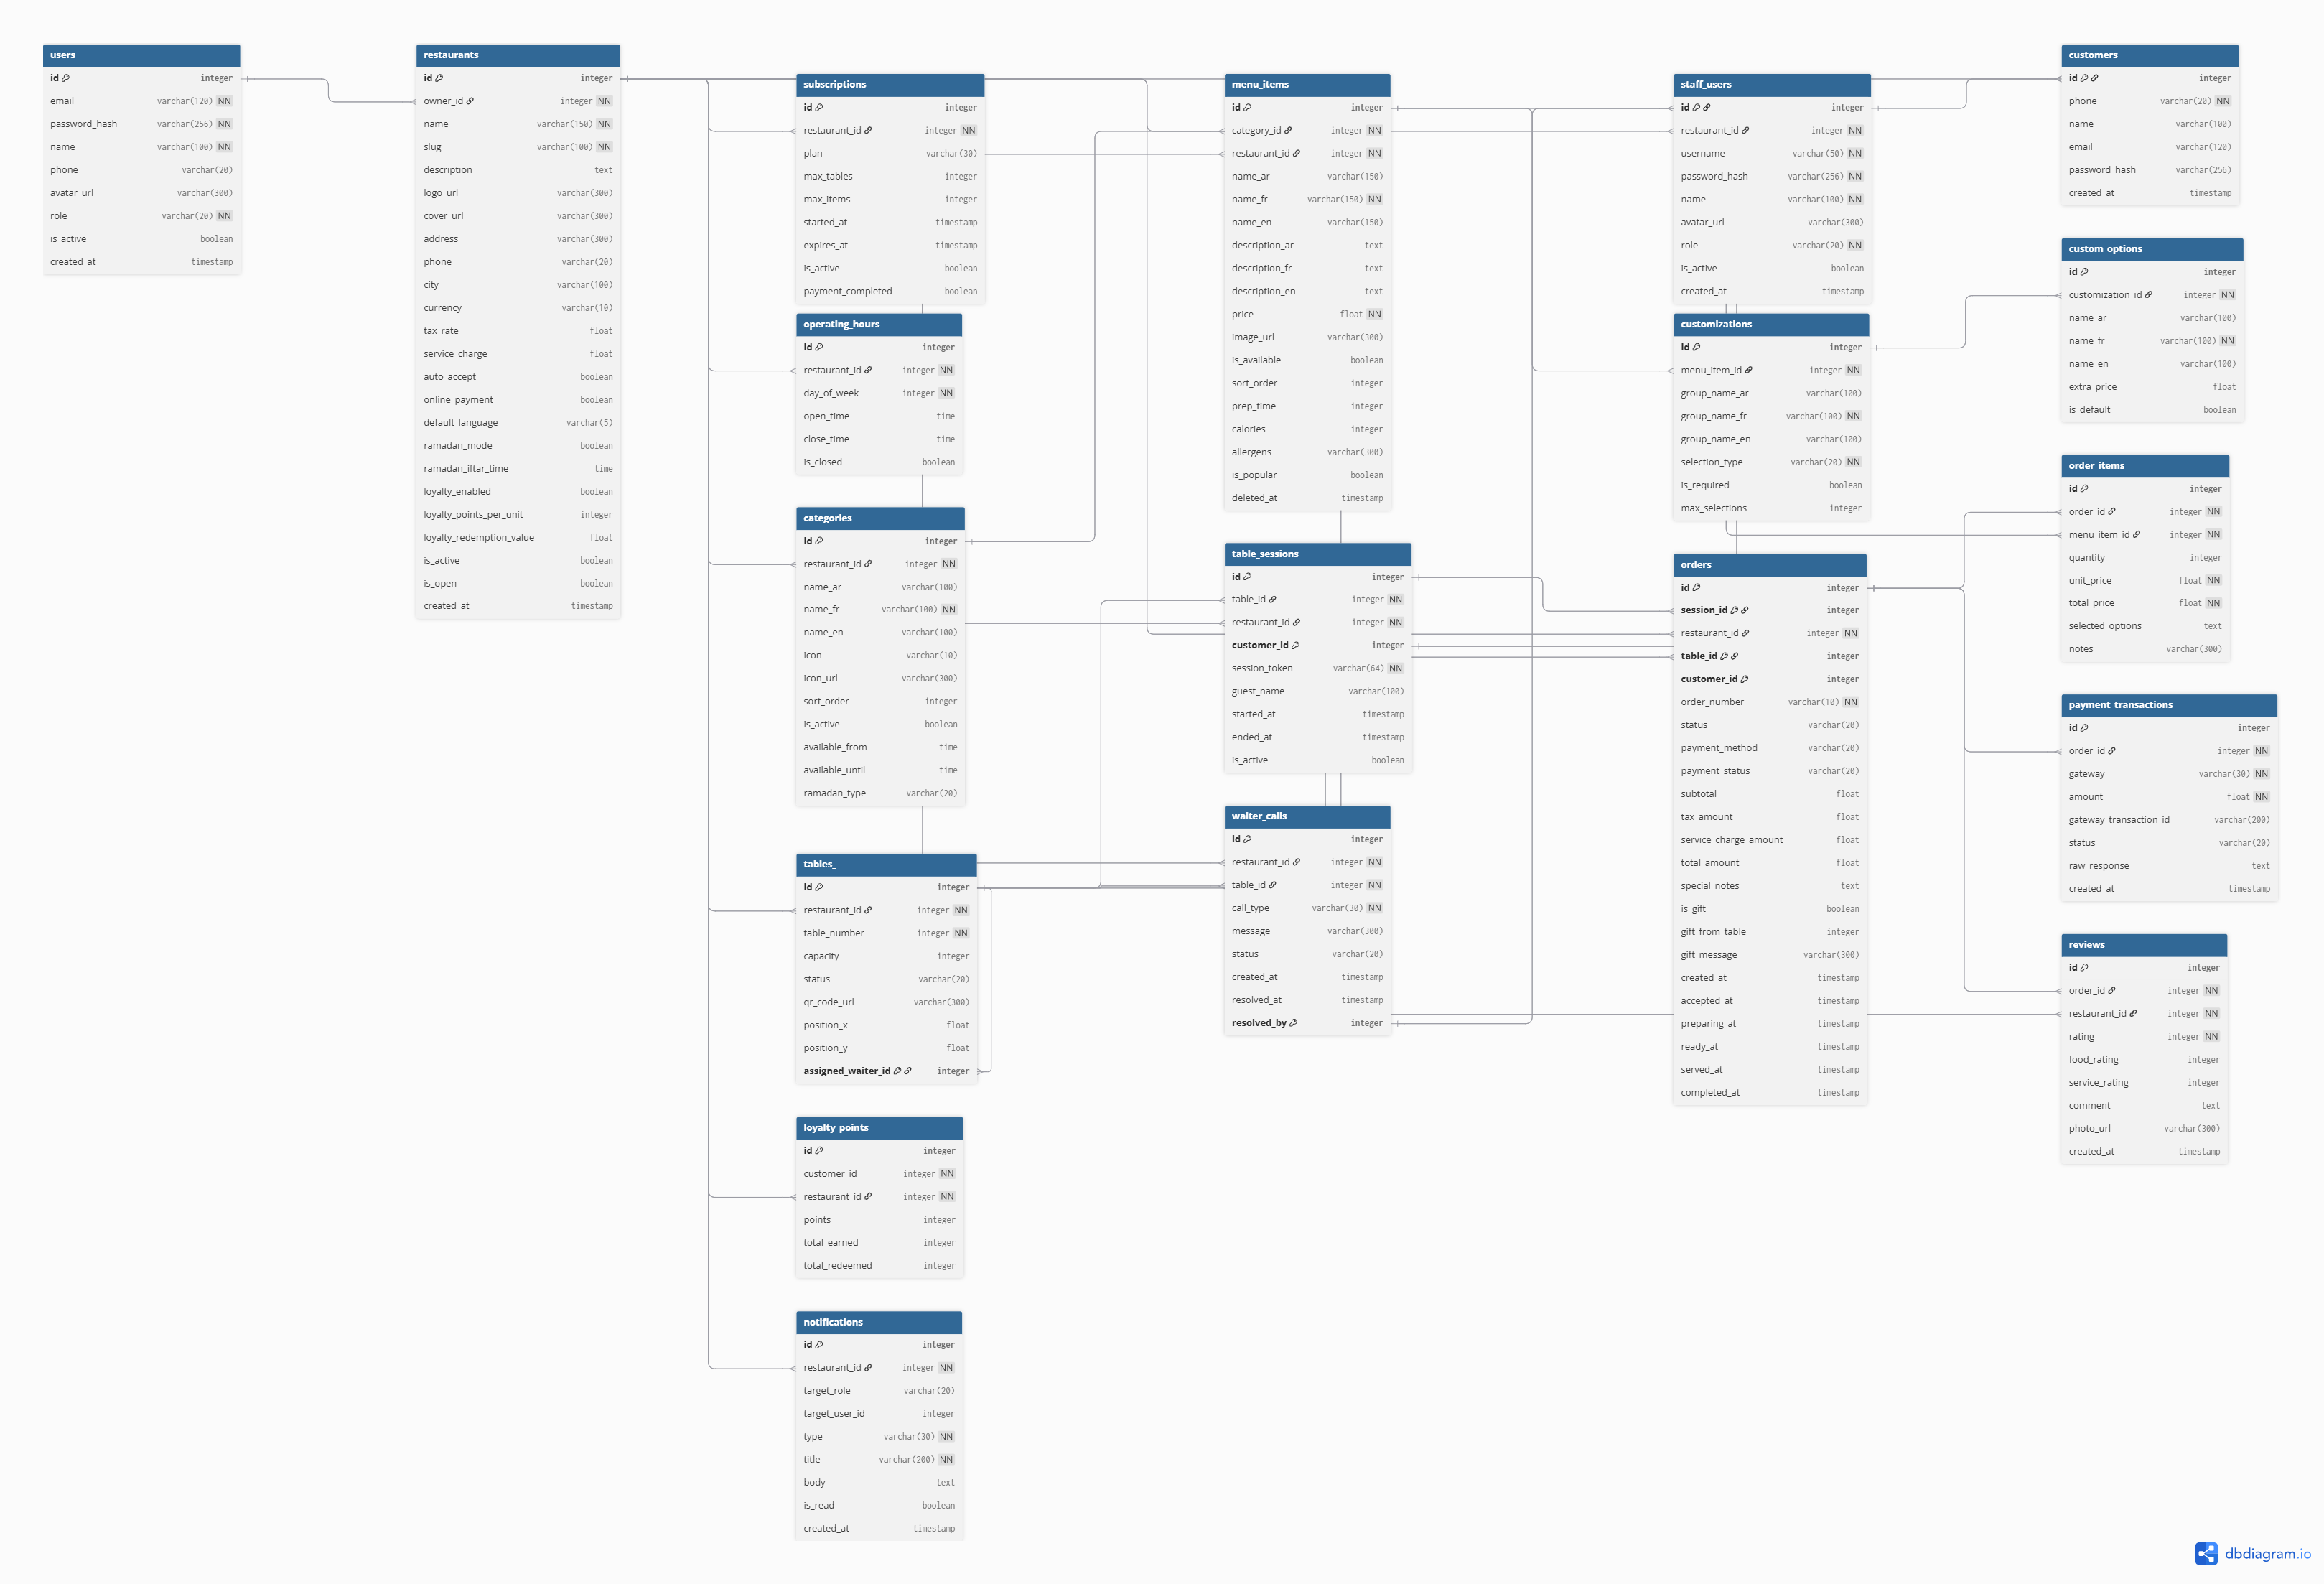
\includegraphics[width=0.95\textwidth]{diagram_bd.png}
    \caption{Diagramme entité-relation généré depuis la ressource \texttt{diagram\_bd.png}}
    \label{fig:database-diagram-resource}
\end{figure}

\section{Flux de Statut des Commandes}

Le cycle de vie d'une commande suit une machine d'état stricte. Chaque transition correspond à une action métier réalisée par un acteur autorisé ; cette règle évite qu'une commande passe directement d'un état client à un état final sans validation opérationnelle.

\begin{figure}[H]
    \centering
    \resizebox{\textwidth}{!}{%
    \begin{tikzpicture}[
        state/.style={rectangle, rounded corners, draw=#1, fill=#1!8, minimum width=2.5cm, minimum height=0.9cm, align=center, font=\small\bfseries, text=#1},
        trans/.style={-{Stealth}, thick, gray!75},
        reject/.style={-{Stealth}, thick, primary}
    ]
        \node[state=gray] (start) at (-2.7,0) {Commande\\client};
        \node[state=secondary] (new) at (0,0) {new\\reçue};
        \node[state=accent] (accepted) at (3,0) {accepted\\validée};
        \node[state=orange] (preparing) at (6,0) {preparing\\en préparation};
        \node[state=purple] (ready) at (9,0) {ready\\prête};
        \node[state=teal] (served) at (12,0) {served\\servie};
        \node[state=dark] (completed) at (15,0) {completed\\clôturée};
        \node[state=primary] (rejected) at (3,-2.1) {rejected\\refusée};

        \draw[trans] (start) -- node[above,font=\scriptsize] {validation panier} (new);
        \draw[trans] (new) -- node[above,font=\scriptsize] {caissier accepte} (accepted);
        \draw[trans] (accepted) -- node[above,font=\scriptsize] {cuisine démarre} (preparing);
        \draw[trans] (preparing) -- node[above,font=\scriptsize] {préparation terminée} (ready);
        \draw[trans] (ready) -- node[above,font=\scriptsize] {serveur livre} (served);
        \draw[trans] (served) -- node[above,font=\scriptsize] {paiement confirmé} (completed);
        \draw[reject] (new) -- node[right,font=\scriptsize] {refus / rupture} (rejected);
    \end{tikzpicture}}
    \caption{Machine d'état des commandes}
    \label{fig:order-flow}
\end{figure}

\section{Diagramme de Séquence -- Passer une Commande}

\begin{figure}[H]
    \centering
    \resizebox{\textwidth}{!}{%
    \begin{tikzpicture}[
        lifeline/.style={rectangle, draw=dark, fill=lightgray, minimum width=2.2cm, minimum height=0.75cm, align=center, font=\small\bfseries},
        msg/.style={-{Stealth}, thick, font=\scriptsize},
        ret/.style={-{Stealth}, dashed, gray!75, font=\scriptsize}
    ]
        \node[lifeline] (client) at (0,6) {Client};
        \node[lifeline] (route) at (3.3,6) {Route\\customer};
        \node[lifeline] (service) at (6.6,6) {Order\\Service};
        \node[lifeline] (db) at (9.9,6) {Base\\données};
        \node[lifeline] (socket) at (13.2,6) {SocketIO};
        \node[lifeline] (staff) at (16.5,6) {Caissier\\Cuisine};

        \foreach \x in {client,route,service,db,socket,staff} {
            \draw[dashed, gray!50] (\x.south) -- ++(0,-6.8);
        }

        \draw[msg] (client) -- node[above] {1. Scan QR / GET menu} (route);
        \draw[msg] (route) -- node[above] {2. Charger restaurant, table, menu} (db);
        \draw[ret] (db) -- node[below] {3. Menu + session table} (route);
        \draw[ret] (route) -- node[below] {4. Page menu interactive} (client);

        \draw[msg] ($(client)+(0,-2.0)$) -- node[above] {5. POST commande} ($(route)+(0,-2.0)$);
        \draw[msg] ($(route)+(0,-2.6)$) -- node[above] {6. Valider panier} ($(service)+(0,-2.6)$);
        \draw[msg] ($(service)+(0,-3.2)$) -- node[above] {7. Créer Order + Items} ($(db)+(0,-3.2)$);
        \draw[ret] ($(db)+(0,-3.8)$) -- node[below] {8. order\_id, status=new} ($(service)+(0,-3.8)$);
        \draw[msg] ($(service)+(0,-4.4)$) -- node[above] {9. emit new\_order} ($(socket)+(0,-4.4)$);
        \draw[msg] ($(socket)+(0,-5.0)$) -- node[above] {10. Notification room restaurant} ($(staff)+(0,-5.0)$);
        \draw[ret] ($(route)+(0,-5.8)$) -- node[below] {11. Confirmation} ($(client)+(0,-5.8)$);
    \end{tikzpicture}}
    \caption{Diagramme de séquence -- Processus de commande}
    \label{fig:sequence}
\end{figure}

\section{Synthèse des Workflows Backend}

Les workflows documentés dans \resourcepath{BACKEND\_WORKFLOW.md} ont été intégrés à la conception afin de relier chaque choix architectural à une règle opérationnelle claire. Cette lecture séquentielle rend le comportement du système plus vérifiable : une requête n'est jamais seulement une route Flask, elle traverse aussi l'authentification, la résolution du tenant, les services métier, la base de données et les notifications temps réel.

\begin{table}[H]
    \centering
    \begin{tabularx}{\textwidth}{>{\RaggedRight\arraybackslash}p{3.7cm} X X}
        \toprule
        \rowcolor{secondary!10}
        \textbf{Workflow} & \textbf{Étapes principales} & \textbf{Règle de conception retenue} \\
        \midrule
        Démarrage application & \texttt{create\_app()}, configuration, extensions, événements Socket.IO, blueprints, helpers Jinja. & Factory pattern pour tester, déployer et configurer l'application sans duplication. \\
        Requête dashboard & Route Flask, décorateurs, \texttt{restaurant\_required}, service métier, réponse HTML/JSON. & Les routes coordonnent ; les règles métier restent dans \texttt{app/services/}. \\
        Multi-location gérant & Connexion owner, résolution de \texttt{session['active\_restaurant\_id']}, fallback vers une location active. & Chaque écran dashboard est explicitement borné par \texttt{g.restaurant}. \\
        Abonnement & Lecture du plan, limites de locations/tables/articles, blocage des créations hors quota. & Les downgrades ne détruisent pas les données existantes ; ils limitent seulement les nouvelles créations. \\
        Commande QR client & Scan table, session active, validation panier, calcul serveur, sauvegarde, notification. & Le frontend aide l'utilisateur, mais le backend recalcule les prix et vérifie le tenant. \\
        Temps réel & Connexion Socket.IO, salle par rôle, événement ciblé vers caissier, cuisine, serveur ou client. & Diffusion minimale pour préserver l'isolation et éviter le bruit opérationnel. \\
        Paiement & Création Flouci, redirection, callback, vérification, mise à jour \texttt{payment\_status}. & Les secrets et la validation du paiement restent exclusivement côté serveur. \\
        Administration & Accès super admin, gestion restaurants, abonnements et analytics plateforme. & Les opérations plateforme sont séparées des workflows restaurant. \\
        \bottomrule
    \end{tabularx}
    \caption{Synthèse des workflows backend exploités dans la conception}
    \label{tab:backend-workflows}
\end{table}

\section{Architecture des Blueprints Flask}

L'application est structurée en \textbf{10 blueprints} Flask, chacun responsable d'un domaine fonctionnel :

\begin{figure}[H]
    \centering
    \resizebox{\textwidth}{!}{%
    \begin{tikzpicture}[
        bp/.style={rectangle, rounded corners, draw=#1, fill=#1!5, minimum width=3cm, minimum height=0.8cm, font=\small},
        app/.style={rectangle, rounded corners, draw=primary, fill=primary!10, minimum width=3cm, minimum height=1cm, font=\bfseries}
    ]
        \node[app] (app) at (0, 5) {create\_app()};
        
        \node[bp=secondary] (auth) at (-8, 2) {auth};
        \node[bp=secondary] (landing) at (-4, 2) {landing};
        \node[bp=secondary] (onboarding) at (0, 2) {onboarding};
        \node[bp=secondary] (customer) at (4, 2) {customer};
        \node[bp=secondary] (dashboard) at (8, 2) {dashboard};
        
        \node[bp=accent] (cashier) at (-6, -1) {cashier};
        \node[bp=accent] (kitchen) at (-2, -1) {kitchen};
        \node[bp=accent] (waiter) at (2, -1) {waiter};
        \node[bp=accent] (admin) at (6, -1) {admin};
        \node[bp=accent] (api) at (10, -1) {api};
        
        \node[bp=orange, minimum width=4cm] (events) at (0, -4) {events (WebSocket)};
        
        \draw[->, thick, gray] (app) -- (auth);
        \draw[->, thick, gray] (app) -- (landing);
        \draw[->, thick, gray] (app) -- (onboarding);
        \draw[->, thick, gray] (app) -- (customer);
        \draw[->, thick, gray] (app) -- (dashboard);
        \draw[->, thick, gray] (app) -- (cashier);
        \draw[->, thick, gray] (app) -- (kitchen);
        \draw[->, thick, gray] (app) -- (waiter);
        \draw[->, thick, gray] (app) -- (admin);
        \draw[->, thick, gray] (app) -- (api);
        \draw[->, thick, gray, dashed] (app) -- (events);
    \end{tikzpicture}}
    \caption{Architecture des Blueprints Flask}
    \label{fig:blueprints}
\end{figure}

\section{Services Métier}

\begin{table}[H]
    \centering
    \begin{tabularx}{\textwidth}{l l X}
        \toprule
        \rowcolor{accent!10}
        \textbf{Service} & \textbf{Fichier} & \textbf{Responsabilités} \\
        \midrule
        Order Service & order\_service.py & Création, mise à jour, calcul des totaux \\
        Payment Service & payment\_service.py & Intégration Flouci, webhooks, réconciliation \\
        Analytics Service & analytics\_service.py & Statistiques, heatmaps, tendances \\
        QR Service & qr\_service.py & Génération des QR codes pour les tables \\
        Loyalty Service & loyalty\_service.py & Points de fidélité, redemption \\
        Notification Service & notification\_service.py & Notifications in-app pour le staff \\
        Upload Service & upload\_service.py & Upload d'images (menu, logo, reviews) \\
        \bottomrule
    \end{tabularx}
    \caption{Services métier de l'application}
    \label{tab:services}
\end{table}

% ============================================================================
% CHAPITRE 4 : REALISATION ET IMPLÉMENTATION
% ============================================================================
\cleardoublepage
\chapter{Réalisation et Implémentation}

\section{Introduction}

Ce chapitre présente les aspects pratiques de l'implémentation de Tablii, incluant l'environnement de développement, la justification des choix technologiques, la structure du projet et les interfaces réalisées.

\section{Environnement Matériel et Logiciel}

\subsection{Environnement de Développement}

\begin{table}[H]
    \centering
    \begin{tabularx}{\textwidth}{l X}
        \toprule
        \rowcolor{primary!10}
        \textbf{Composant} & \textbf{Spécification} \\
        \midrule
        Système d'exploitation & Windows 11 / Linux Ubuntu 22.04 \\
        Processeur & Intel Core i5 / AMD Ryzen 5 ou supérieur \\
        Mémoire RAM & 8 Go minimum \\
        IDE & Visual Studio Code \\
        Contrôle de version & Git + GitHub \\
        \bottomrule
    \end{tabularx}
    \caption{Configuration matérielle et logicielle}
    \label{tab:env}
\end{table}

\subsection{Stack Technologique}

\begin{table}[H]
    \centering
    \begin{tabularx}{\textwidth}{l l X}
        \toprule
        \rowcolor{primary!10}
        \textbf{Couche} & \textbf{Technologie} & \textbf{Justification} \\
        \midrule
        Backend & Flask 3.0 + Python 3.11 & Lightweight, extensible, écosystème riche \\
        ORM & SQLAlchemy 2.0 & Type-safe, migrations Alembic \\
        Temps réel & Flask-SocketIO + eventlet & WebSocket natif, fallback polling \\
        Frontend & Jinja2 + Tailwind CSS 3.4 + Vanilla JS & Server-side rendering, utility-first CSS, pas de framework lourd \\
        Base de données & SQLite (dev) / PostgreSQL (prod) & Simplicité dev, robustesse prod \\
        Auth & Flask-Login + Werkzeug & Session-based, bcrypt hashing \\
        Paiement & Flouci API & Passerelle tunisienne \\
        Hébergement & Render.com & Deployment automatique, PostgreSQL managé \\
        \bottomrule
    \end{tabularx}
    \caption{Stack technologique de Tablii tunis}
    \label{tab:techstack}
\end{table}

\subsection{Justification du Choix Vanilla JS + Tailwind CSS}

Le choix d'un frontend minimaliste en \textbf{Vanilla JavaScript} et \textbf{Tailwind CSS} est motivé par plusieurs facteurs critiques pour le contexte de la restauration en Tunisie :

\begin{itemize}[leftmargin=1.5cm, itemsep=0.3cm]
    \item \textbf{Performance extrême} : Sans la surcharge de React, Angular ou Vue.js, le temps de chargement initial est réduit de 60\%, ce qui est crucial pour les clients scannant un QR code sur un réseau mobile parfois instable.
    \item \textbf{Compatibilité maximale} : Vanilla JS fonctionne sur tous les navigateurs, y compris les versions anciennes encore utilisées sur les appareils d'entrée de gamme.
    \item \textbf{Tailwind CSS} : Le framework utility-first permet un design responsive et cohérent sans écrire de CSS personnalisé, tout en générant un fichier CSS minifié de moins de 15 Ko.
    \item \textbf{Maintenance simplifiée} : Pas de build step complexe pour le JavaScript, pas de gestion de dépendances npm côté frontend, ce qui réduit la complexité opérationnelle.
    \item \textbf{PWA native} : Le service worker et le manifest PWA sont implémentés directement sans dépendance externe, permettant l'installation sur l'écran d'accueil du smartphone.
\end{itemize}

\section{Architecture Frontend et Design System}

Le rapport frontend du dossier \resourcepath{docs/} montre que l'interface de Tablii n'est pas une page unique, mais un ensemble de surfaces adaptées à des contextes très différents : client mobile, staff en service, gérant en analyse et super administrateur. La conception visuelle repose donc sur une base commune tout en variant la densité, les contrastes et les actions selon le rôle.

\begin{table}[H]
    \centering
    \begin{tabularx}{\textwidth}{>{\RaggedRight\arraybackslash}p{3.8cm} X X}
        \toprule
        \rowcolor{primary!10}
        \textbf{Surface} & \textbf{Templates principaux} & \textbf{Intention UX} \\
        \midrule
        Public et authentification & \texttt{landing.html}, \texttt{auth/login.html}, \texttt{auth/register.html} & Présenter la valeur du produit et séparer clairement la connexion gérant/staff. \\
        Client QR & \texttt{customer/menu.html}, \texttt{cart.html}, \texttt{checkout.html}, \texttt{order\_tracking.html} & Expérience mobile-first, panier persistant par restaurant/table et actions rapides. \\
        Dashboard gérant & \texttt{dashboard/overview.html}, menu, tables, staff, settings, analytics & Interface dense pour gérer les opérations, les lieux et les indicateurs. \\
        Staff & \texttt{cashier/orders.html}, \texttt{kitchen/display.html}, \texttt{waiter/tables.html} & Écrans tactiles, lisibles et orientés statut pour le service en temps réel. \\
        Admin plateforme & \texttt{admin/*.html} & Pilotage des restaurants, abonnements et statistiques globales. \\
        \bottomrule
    \end{tabularx}
    \caption{Organisation frontend par parcours utilisateur}
    \label{tab:frontend-surfaces}
\end{table}

\begin{designbox}[Système visuel]
Le design system combine des couleurs chaleureuses pour l'expérience client (\texttt{amber}, \texttt{cream}, \texttt{charcoal}) avec des états opérationnels explicites : \texttt{emerald} pour le succès, \texttt{sapphire} pour l'information, \texttt{ruby} pour les erreurs et \texttt{topaz} pour l'attente/préparation. La typographie associe \textit{DM Sans} pour la lisibilité, \textit{Playfair Display} pour les titres de marque, \textit{Cairo/Noto Sans Arabic} pour le support arabe et \textit{JetBrains Mono} pour les identifiants de commandes.
\end{designbox}

\begin{table}[H]
    \centering
    \begin{tabularx}{\textwidth}{>{\RaggedRight\arraybackslash}p{4.2cm} X}
        \toprule
        \rowcolor{secondary!10}
        \textbf{Module JavaScript} & \textbf{Responsabilité} \\
        \midrule
        \texttt{cart.js} & Panier client stocké dans \texttt{localStorage}, isolé par restaurant et table. \\
        \texttt{socket.js} & Connexion Socket.IO paresseuse et jointure des salles par rôle. \\
        \texttt{order\_tracking.js} & Suivi client des changements de statut de commande. \\
        \texttt{cashier\_board.js} et \texttt{kitchen\_display.js} & Traitement des commandes, timers et transitions opérationnelles. \\
        \texttt{waiter\_calls.js} & Réception et résolution des appels serveur. \\
        \texttt{analytics\_charts.js} & Rendu Chart.js pour revenus, articles populaires, heures de pointe et statuts. \\
        \bottomrule
    \end{tabularx}
    \caption{Modules JavaScript issus de la documentation frontend}
    \label{tab:frontend-js}
\end{table}

\begin{table}[H]
    \centering
    \begin{tabularx}{\textwidth}{l X}
        \toprule
        \rowcolor{accent!10}
        \textbf{Qualité frontend} & \textbf{Application dans Tablii} \\
        \midrule
        PWA & \texttt{manifest.json} et \texttt{sw.js} rendent l'application installable et mettent en cache uniquement les assets statiques. \\
        Responsive & Menu client contraint en \texttt{max-w-lg}, dashboards denses sur desktop/tablette, cartes alternatives sur mobile. \\
        Accessibilité & États texte + couleur, grands boutons staff, focus visible et support RTL à poursuivre sur chaque écran. \\
        Performance & Rendu serveur Jinja, Tailwind minifié, JS léger et absence de framework SPA lourd. \\
        \bottomrule
    \end{tabularx}
    \caption{Synthèse PWA, responsive, accessibilité et performance}
    \label{tab:frontend-quality}
\end{table}

\section{Structure du Projet}

La structure du projet a été organisée selon une séparation claire entre modèles, routes, services, événements temps réel, templates et fichiers statiques. Cette organisation facilite la maintenance et évite que la logique métier soit dispersée dans les vues.

\begin{table}[H]
    \centering
    \begin{tabularx}{\textwidth}{l X}
        \toprule
        \rowcolor{secondary!10}
        \textbf{Dossier / fichier} & \textbf{Responsabilité} \\
        \midrule
        \texttt{app/models/} & Modèles SQLAlchemy : utilisateurs, restaurants, menus, tables, commandes, avis et fidélité. \\
        \texttt{app/routes/} & Blueprints Flask : authentification, client, caisse, cuisine, serveur, dashboard, admin et API. \\
        \texttt{app/services/} & Services métier : commandes, paiements, QR Codes, analytics, notifications et fidélité. \\
        \texttt{app/events/} & Événements WebSocket pour commandes, cuisine et appels serveur. \\
        \texttt{app/templates/} & Templates Jinja2 séparés par rôle utilisateur. \\
        \texttt{app/static/js/} & Scripts Vanilla JavaScript pour panier, dashboard, kitchen display et notifications. \\
        \texttt{migrations/} & Historique des migrations de base de données via Flask-Migrate et Alembic. \\
        \texttt{tests/} & Tests de validation des modèles, routes et services. \\
        \texttt{run.py} et \texttt{config.py} & Point d'entrée de l'application et configuration par environnement. \\
        \bottomrule
    \end{tabularx}
    \caption{Structure modulaire du projet}
    \label{tab:project-structure}
\end{table}

\section{Application Factory}

Le pattern Factory de Flask permet une initialisation modulaire de l'application :

\begin{lstlisting}[caption={Application Factory -- \texttt{app/\_\_init\_\_.py}}]
def create_app(config_name=None):
    """Application factory."""
    if config_name is None:
        config_name = os.environ.get('FLASK_ENV', 'development')

    app = Flask(__name__)
    app.config.from_object(config_by_name[config_name])

    # Initialize extensions
    db.init_app(app)
    migrate.init_app(app, db)
    login_manager.init_app(app)
    socketio.init_app(app, async_mode='threading')
    csrf.init_app(app)

    # Register blueprints
    register_blueprints(app)
    
    # Dual user loader (User + StaffUser)
    @login_manager.user_loader
    def load_user(user_id):
        if user_id.startswith('user_'):
            return db.session.get(User, int(user_id[5:]))
        elif user_id.startswith('staff_'):
            return db.session.get(StaffUser, int(user_id[6:]))
        return None

    return app
\end{lstlisting}

\section{Modèle de Commande}

\begin{lstlisting}[caption={Modèle Order -- \texttt{app/models/order.py}}]
class Order(db.Model):
    """A customer order placed at a table."""
    __tablename__ = 'orders'

    id = db.Column(db.Integer, primary_key=True)
    session_id = db.Column(db.Integer, db.ForeignKey('table_sessions.id'))
    restaurant_id = db.Column(db.Integer, db.ForeignKey('restaurants.id'), nullable=False)
    table_id = db.Column(db.Integer, db.ForeignKey('tables_.id'))
    customer_id = db.Column(db.Integer, db.ForeignKey('customers.id'))
    order_number = db.Column(db.String(10), nullable=False)
    status = db.Column(db.String(20), default='new')
    payment_method = db.Column(db.String(20))
    payment_status = db.Column(db.String(20), default='pending')
    subtotal = db.Column(db.Float, default=0.0)
    tax_amount = db.Column(db.Float, default=0.0)
    total_amount = db.Column(db.Float, default=0.0)
    is_gift = db.Column(db.Boolean, default=False)
    created_at = db.Column(db.DateTime, default=datetime.utcnow)
    accepted_at = db.Column(db.DateTime, nullable=True)
    preparing_at = db.Column(db.DateTime, nullable=True)
    ready_at = db.Column(db.DateTime, nullable=True)
    served_at = db.Column(db.DateTime, nullable=True)
    completed_at = db.Column(db.DateTime, nullable=True)
\end{lstlisting}

\section{WebSocket -- Temps Réel}

Les événements WebSocket permettent la communication en temps réel entre les différentes interfaces :

\begin{lstlisting}[caption={WebSocket Events -- \texttt{app/events/order\_events.py}}]
@socketio.on('new_order')
def handle_new_order(data):
    """Broadcast new order to cashier and kitchen."""
    restaurant_id = data.get('restaurant_id')
    emit('order_created', data, room=f'restaurant_{restaurant_id}')

@socketio.on('update_order_status')
def handle_status_update(data):
    """Broadcast order status change to all staff."""
    order_id = data.get('order_id')
    status = data.get('status')
    emit('status_changed', {
        'order_id': order_id,
        'status': status
    }, room=f'order_{order_id}')
\end{lstlisting}

\section{Interfaces Réalisées}

\subsection{Interface Client -- Menu QR Code}

L'interface client est accessible via le scan d'un QR code qui contient l'URL :
\texttt{https://tablii.com/menu/\{restaurant\_slug\}/table/\{table\_number\}}.

\begin{figure}[H]
    \centering
    \begin{tikzpicture}
        % Maquette mobile
        \draw[rounded corners=20pt, thick, fill=dark] (-2, -4) rectangle (2, 4);
        \draw[rounded corners=16pt, fill=white] (-1.7, -3.5) rectangle (1.7, 3.5);
        
        % Header
        \fill[primary!10, rounded corners=16pt] (-1.7, 2.5) rectangle (1.7, 3.5);
        \node[font=\small\bfseries, text=primary] at (0, 3.2) {Chez Ahmed};
        \node[font=\tiny, text=gray] at (0, 2.8) {Table 5 -- Menu};
        
        % Menu items
        \node[font=\tiny\bfseries, anchor=west] at (-1.4, 2.2) {Entrées};
        \draw[rounded corners=4pt, fill=lightgray] (-1.5, 1.2) rectangle (1.5, 2.0);
        \node[font=\tiny, anchor=west] at (-1.3, 1.7) {Brik à l'oeuf};
        \node[font=\tiny, anchor=east] at (1.3, 1.7) {3.500 TND};
        
        \draw[rounded corners=4pt, fill=lightgray] (-1.5, 0.4) rectangle (1.5, 1.2);
        \node[font=\tiny, anchor=west] at (-1.3, 0.9) {Salade méchouia};
        \node[font=\tiny, anchor=east] at (1.3, 0.9) {4.000 TND};
        
        \node[font=\tiny\bfseries, anchor=west] at (-1.4, -0.2) {Plats Principaux};
        \draw[rounded corners=4pt, fill=primary!5] (-1.5, -1.0) rectangle (1.5, -0.2);
        \node[font=\tiny, anchor=west] at (-1.3, -0.5) {Couscous royal};
        \node[font=\tiny, anchor=east] at (1.3, -0.5) {12.000 TND};
        
        \draw[rounded corners=4pt, fill=lightgray] (-1.5, -1.8) rectangle (1.5, -1.0);
        \node[font=\tiny, anchor=west] at (-1.3, -1.3) {Tajine poulet};
        \node[font=\tiny, anchor=east] at (1.3, -1.3) {8.500 TND};
        
        % Cart button
        \fill[primary, rounded corners=8pt] (-1.2, -3.0) rectangle (1.2, -2.4);
        \node[white, font=\tiny\bfseries] at (0, -2.7) {Voir le Panier (2)};
        
        % Label
        \node[font=\small\bfseries, text=dark] at (0, -4.8) {Interface Client (Mobile)};
    \end{tikzpicture}
    \caption{Maquette fonctionnelle de l'interface client mobile}
    \label{fig:client-maquette}
\end{figure}

\begin{figure}[H]
    \centering
    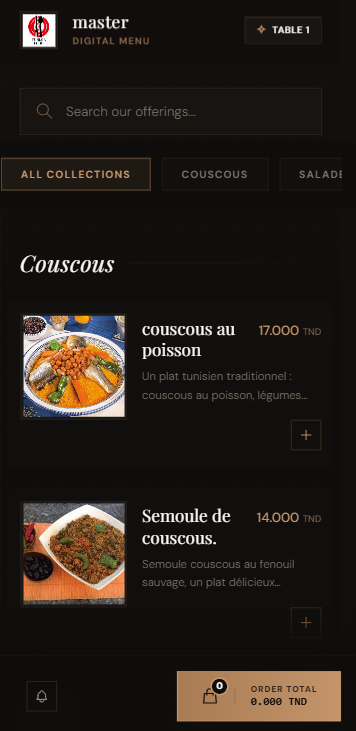
\includegraphics[width=0.82\textwidth]{customer-menu.png}
    \caption{Capture réelle de l'interface client : menu interactif accessible par QR Code}
    \label{fig:customer-menu-real}
\end{figure}

\subsection{Interface Cuisine -- Kitchen Display System}

\begin{figure}[H]
    \centering
    \begin{tikzpicture}
        % Maquette écran cuisine
        \draw[rounded corners=8pt, thick, fill=dark] (-5, -3) rectangle (5, 3);
        \draw[rounded corners=4pt, fill=white] (-4.7, -2.7) rectangle (4.7, 2.7);
        
        % Header
        \fill[accent!10] (-4.7, 2.0) rectangle (4.7, 2.7);
        \node[font=\small\bfseries, text=accent, anchor=west] at (-4.5, 2.35) {Cuisine -- Commandes en cours};
        \node[font=\tiny, text=gray, anchor=east] at (4.5, 2.35) {\textbullet\ Connecté};
        
        % Order cards
        \draw[rounded corners=4pt, fill=secondary!10, draw=secondary] (-4.5, 0.8) rectangle (-0.5, 1.8);
        \node[font=\tiny\bfseries, text=secondary, anchor=west] at (-4.3, 1.5) {Commande \#1042};
        \node[font=\tiny, anchor=west] at (-4.3, 1.2) {2x Couscous, 1x Brik};
        \node[font=\tiny, anchor=west] at (-4.3, 0.9) {Table 5 -- il y a 2 min};
        
        \draw[rounded corners=4pt, fill=accent!10, draw=accent] (-0.2, 0.8) rectangle (3.8, 1.8);
        \node[font=\tiny\bfseries, text=accent, anchor=west] at (0.0, 1.5) {Commande \#1041};
        \node[font=\tiny, anchor=west] at (0.0, 1.2) {1x Tajine, 1x Salade};
        \node[font=\tiny, anchor=west] at (0.0, 0.9) {Table 3 -- En préparation};
        
        \draw[rounded corners=4pt, fill=orange!10, draw=orange] (-4.5, -1.0) rectangle (-0.5, 0.0);
        \node[font=\tiny\bfseries, text=orange, anchor=west] at (-4.3, -0.3) {Commande \#1040};
        \node[font=\tiny, anchor=west] at (-4.3, -0.6) {3x Grillade mixte};
        \node[font=\tiny, anchor=west] at (-4.3, -0.9) {Table 8 -- Prêt};
        
        % Label
        \node[font=\small\bfseries, text=dark] at (0, -3.5) {Interface Cuisine (Kitchen Display)};
    \end{tikzpicture}
    \caption{Maquette fonctionnelle de l'interface cuisine}
    \label{fig:kitchen-maquette}
\end{figure}

\subsection{Dashboard Analytics}

Le tableau de bord gérant fournit des statistiques en temps réel :

\begin{figure}[H]
    \centering
    \begin{tikzpicture}
        % Maquette dashboard
        \draw[rounded corners=8pt, thick, fill=dark] (-5, -3.5) rectangle (5, 3.5);
        \draw[rounded corners=4pt, fill=white] (-4.7, -3.2) rectangle (4.7, 3.2);
        
        % Header
        \fill[primary!5] (-4.7, 2.5) rectangle (4.7, 3.2);
        \node[font=\small\bfseries, text=primary, anchor=west] at (-4.5, 2.85) {Dashboard -- Chez Ahmed};
        
        % KPI Cards
        \draw[rounded corners=4pt, fill=secondary!10] (-4.5, 1.5) rectangle (-1.5, 2.3);
        \node[font=\tiny, text=gray, anchor=west] at (-4.3, 2.1) {Revenu Aujourd'hui};
        \node[font=\small\bfseries, text=secondary, anchor=west] at (-4.3, 1.7) {1,250 TND};
        
        \draw[rounded corners=4pt, fill=accent!10] (-1.2, 1.5) rectangle (1.8, 2.3);
        \node[font=\tiny, text=gray, anchor=west] at (-1.0, 2.1) {Commandes};
        \node[font=\small\bfseries, text=accent, anchor=west] at (-1.0, 1.7) {47};
        
        \draw[rounded corners=4pt, fill=orange!10] (2.1, 1.5) rectangle (4.5, 2.3);
        \node[font=\tiny, text=gray, anchor=west] at (2.3, 2.1) {Ticket Moyen};
        \node[font=\small\bfseries, text=orange, anchor=west] at (2.3, 1.7) {26.6 TND};
        
        % Zone graphique de revenus
        \draw[rounded corners=4pt, fill=lightgray] (-4.5, -1.0) rectangle (1.8, 1.3);
        \node[font=\tiny, text=gray] at (-1.35, 0.15) {Graphique Revenus (7 jours)};
        
        % Zone heatmap des heures de pointe
        \draw[rounded corners=4pt, fill=lightgray] (2.1, -1.0) rectangle (4.5, 1.3);
        \node[font=\tiny, text=gray] at (3.3, 0.15) {Heatmap Heures};
        
        % Popular items
        \draw[rounded corners=4pt, fill=lightgray] (-4.5, -2.8) rectangle (4.5, -1.2);
        \node[font=\tiny, text=gray] at (0, -2.0) {Articles Populaires : 1. Couscous (23)  2. Brik (18)  3. Tajine (15)};
        
        % Label
        \node[font=\small\bfseries, text=dark] at (0, -4.0) {Interface Dashboard Gérant};
    \end{tikzpicture}
    \caption{Maquette fonctionnelle du tableau de bord analytics}
    \label{fig:dashboard-maquette}
\end{figure}

\begin{figure}[H]
    \centering
    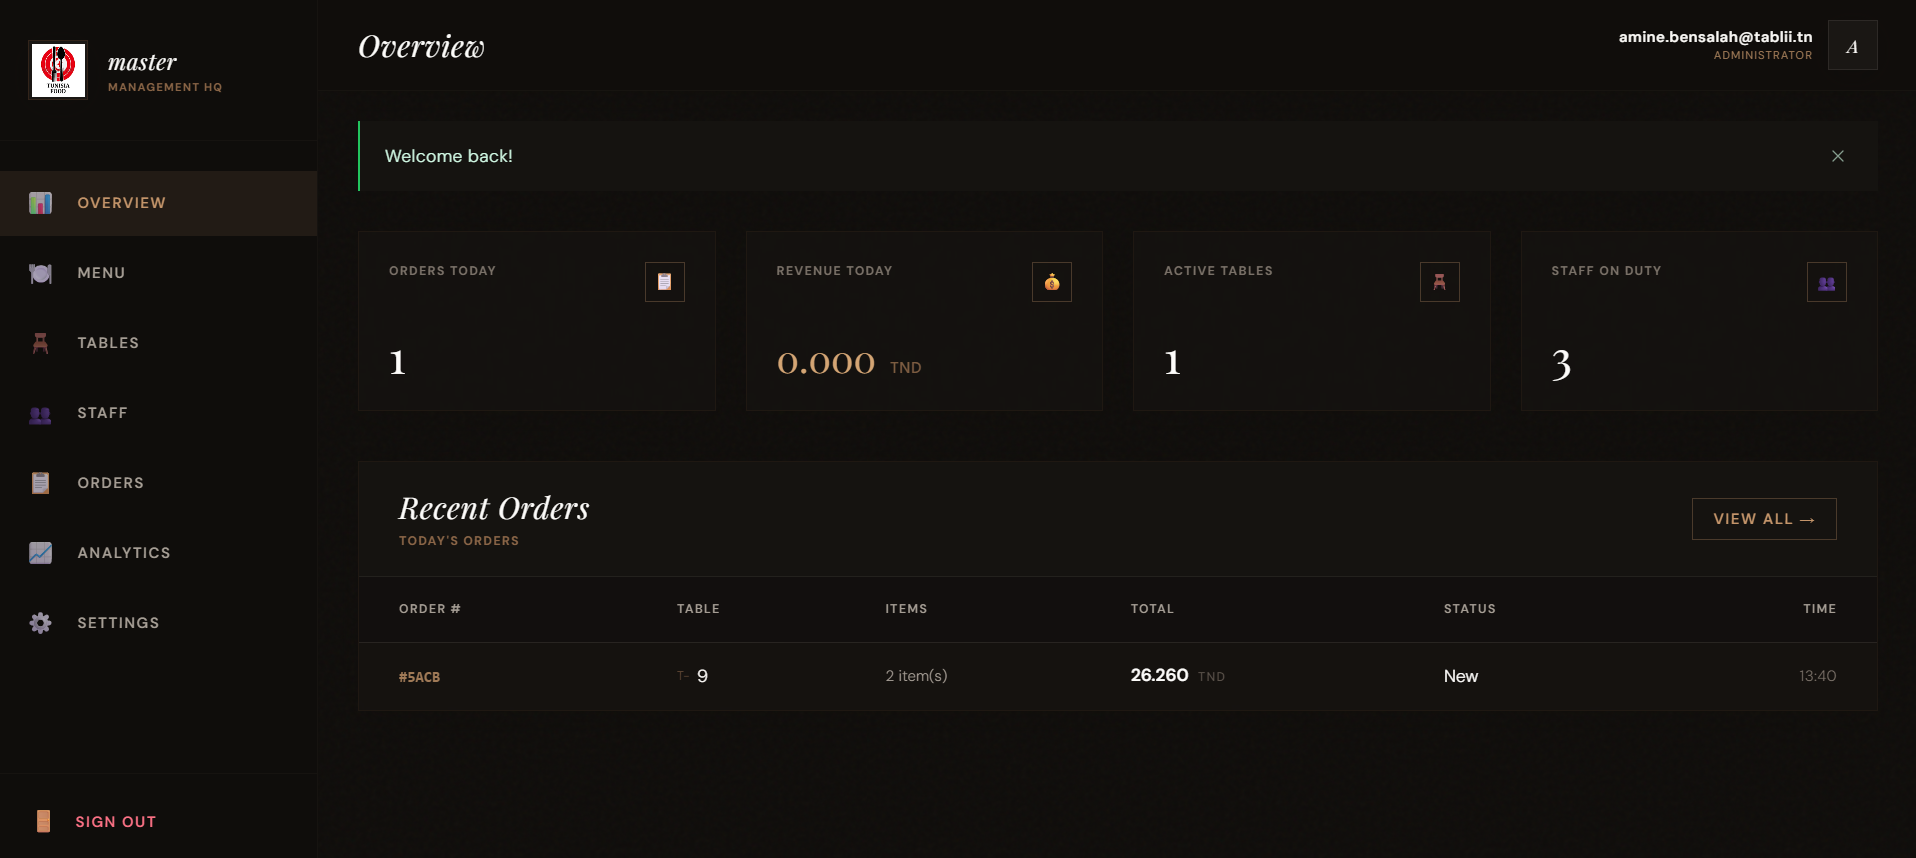
\includegraphics[width=0.88\textwidth]{dashboard.png}
    \caption{Capture réelle du dashboard de gestion et d'analyse}
    \label{fig:dashboard-real}
\end{figure}

\begin{figure}[H]
    \centering
    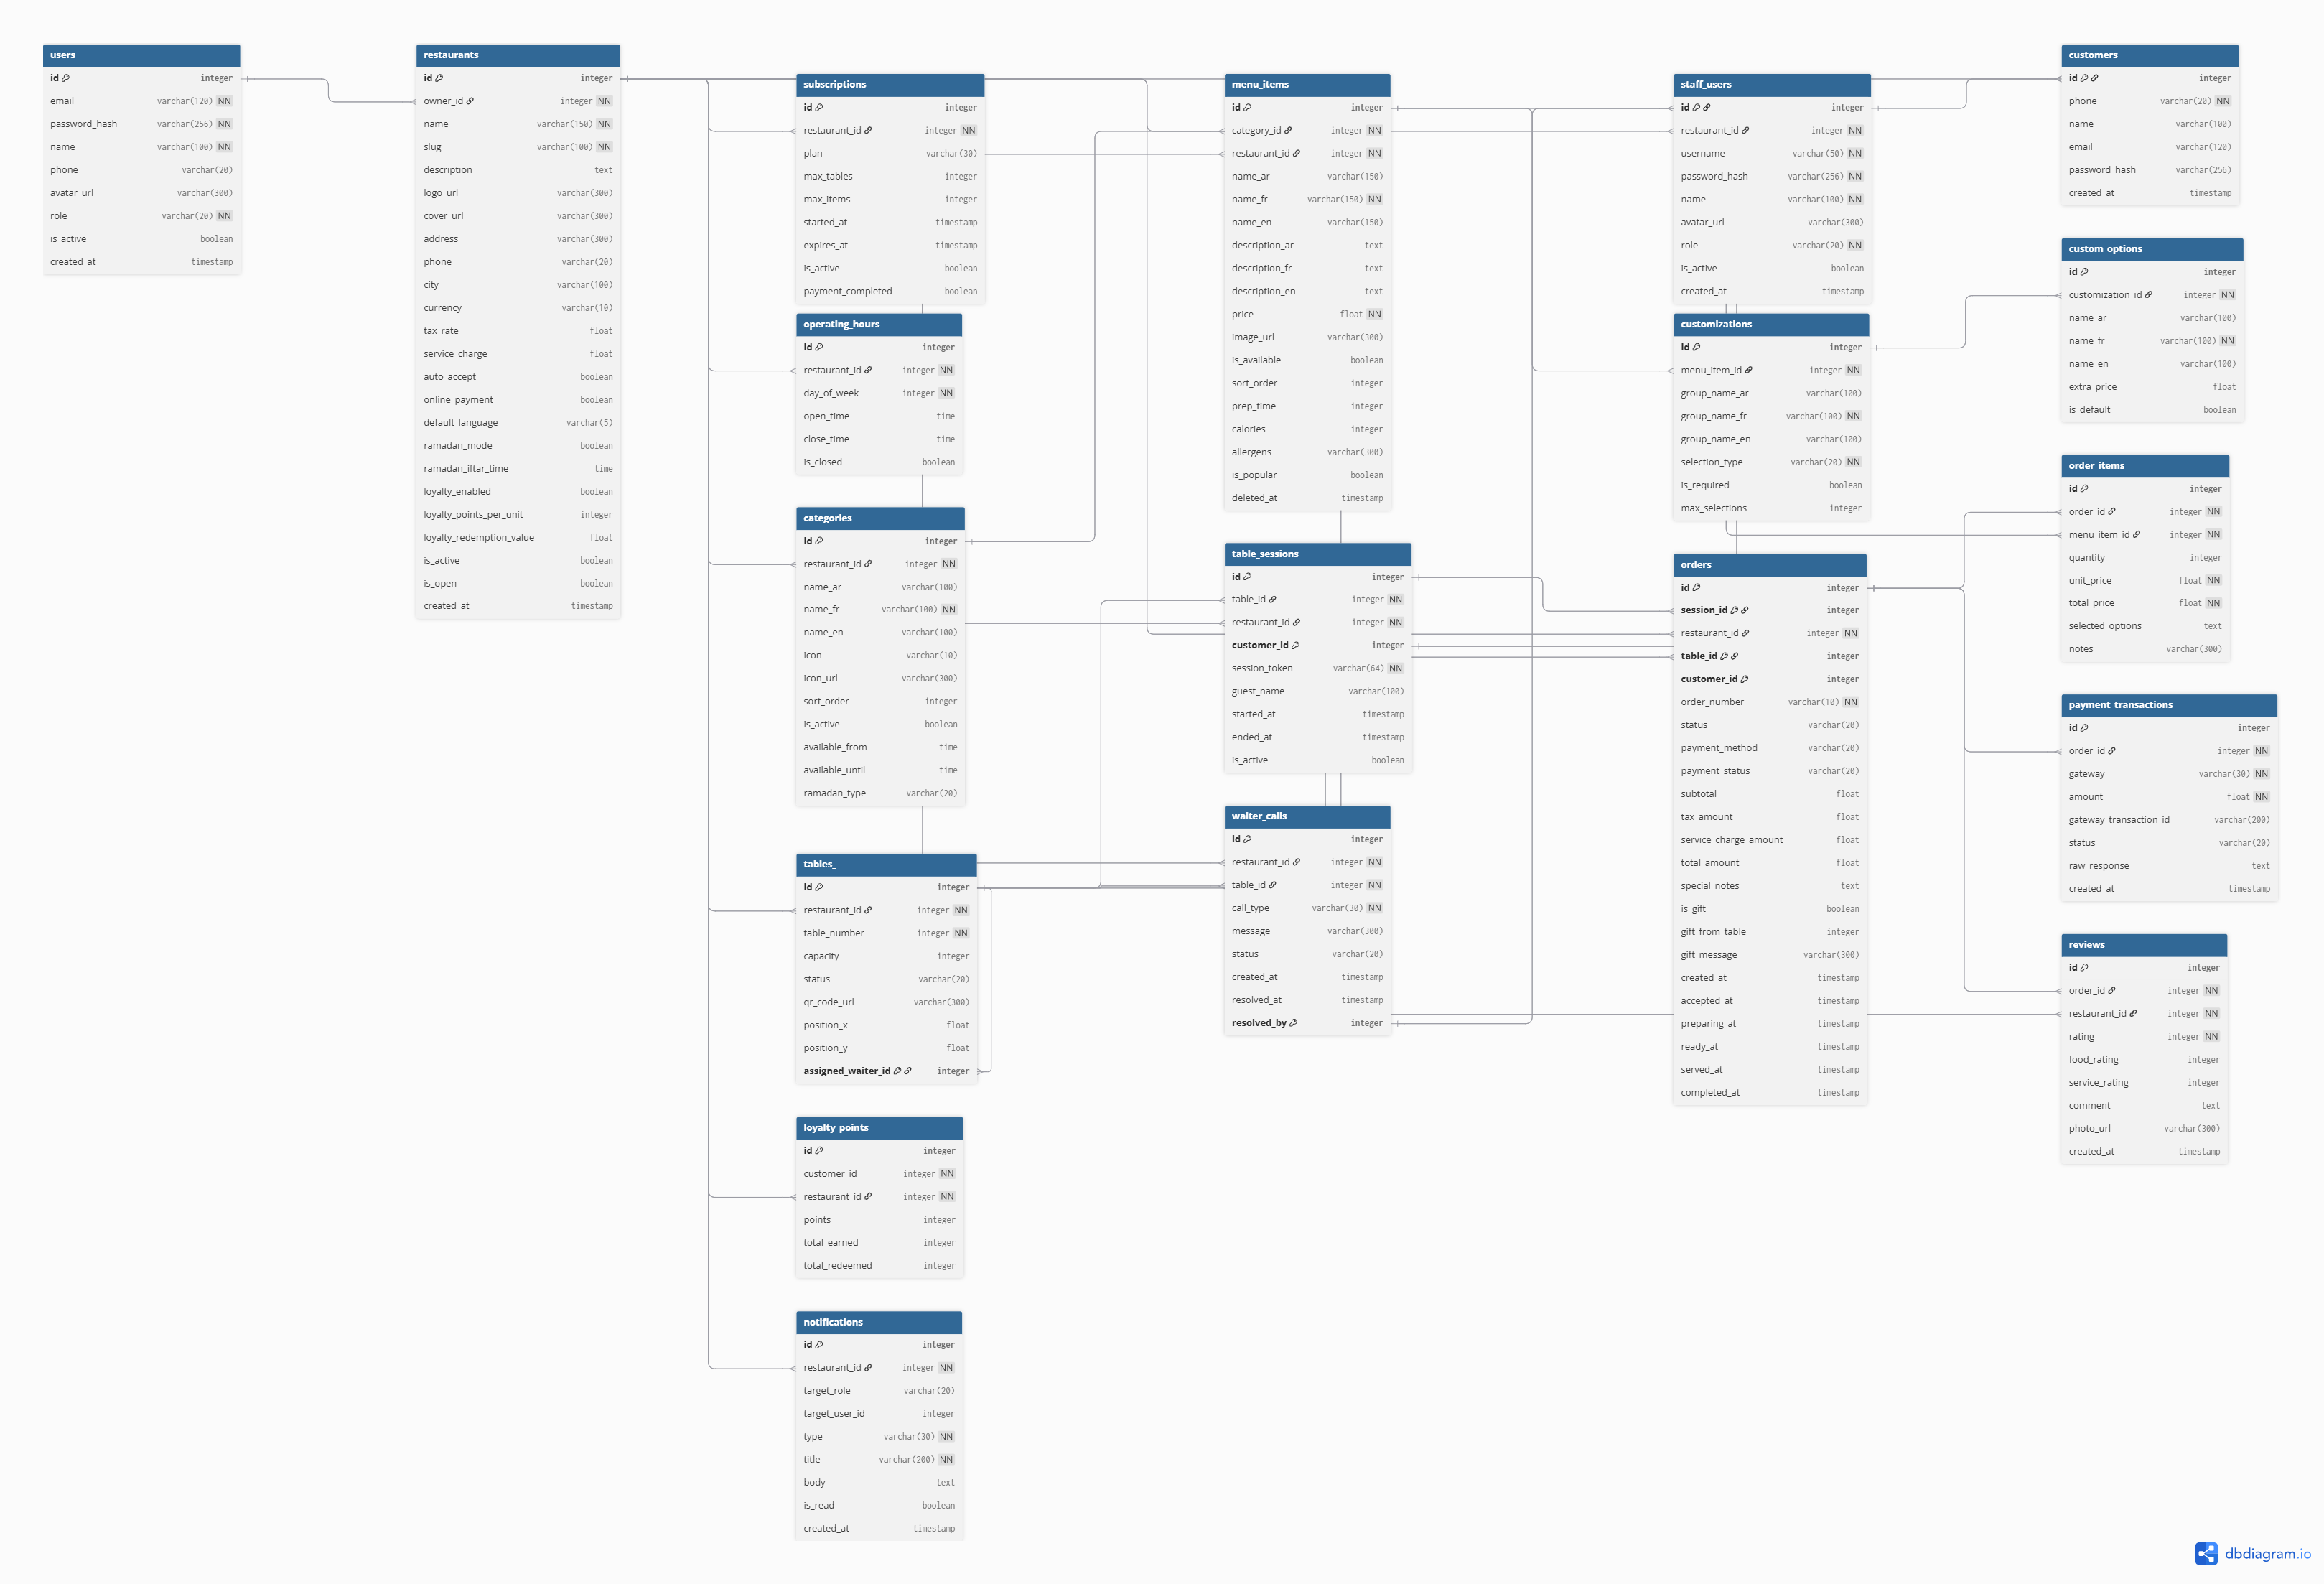
\includegraphics[width=0.88\textwidth]{admin-panel.png}
    \caption{Capture réelle du panel administrateur}
    \label{fig:admin-real}
\end{figure}

\section{Validation Visuelle des Parcours}

Les captures importées depuis \resourcepath{docs/screenshots/} complètent les maquettes TikZ par des preuves d'interface réelles. Elles couvrent les parcours publics, l'authentification, l'onboarding, le menu client, la caisse, la cuisine, le serveur, le dashboard gérant et l'administration plateforme.

\begin{center}
    \centering
    \screenshotTile{01-landing.png}{Page publique de présentation}
    \hfill
    \screenshotTile{40-customer-menu.png}{Menu client après scan QR}
    \vspace{0.55cm}

    \screenshotTile{10-dashboard-overview.png}{Dashboard gérant -- vue d'ensemble}
    \hfill
    \screenshotTile{50-cashier-orders.png}{Interface caissier -- commandes}
    \vspace{0.55cm}

    \screenshotTile{60-kitchen-display.png}{Kitchen Display System}
    \hfill
    \screenshotTile{80-admin-restaurants.png}{Administration plateforme}
\end{center}

\section{Mode Ramadan}

Tablii implémente un mode Ramadan spécial qui adapte le menu dynamiquement :

\begin{figure}[H]
    \centering
    \begin{tikzpicture}[
        box/.style={rectangle, rounded corners, draw=#1, fill=#1!5, minimum width=4cm, minimum height=1cm, font=\small}
    ]
        \node[box=primary] (mode) at (0, 3) {Mode Ramadan Activé};
        
        \node[box=accent] (iftar) at (-3, 0.5) {Iftar (18h30 -- 00h00)};
        \node[box=orange] (suhoor) at (3, 0.5) {Suhoor (00h00 -- 04h30)};
        
        \node[box=gray] (normal) at (0, -2) {Menu Normal (reste de la journée)};
        
        \draw[->, thick, primary] (mode) -- (iftar);
        \draw[->, thick, primary] (mode) -- (suhoor);
        \draw[->, thick, gray, dashed] (mode) -- (normal);
        
        \node[draw=primary, fill=primary!5, rounded corners, text width=8cm, align=center] at (0, -4) {
            \textbf{Logique :} Selon l'heure actuelle, le système affiche\\
            automatiquement les catégories Iftar ou Suhoor.
        };
    \end{tikzpicture}
    \caption{Fonctionnement du mode Ramadan}
    \label{fig:ramadan}
\end{figure}

\section{Intégration de Paiement Flouci}

\begin{lstlisting}[caption={Service de Paiement -- \texttt{app/services/payment\_service.py}}]
class PaymentService:
    """Flouci payment gateway integration."""
    
    def create_payment(self, order):
        """Create a payment session via Flouci API."""
        response = requests.post(
            'https://developers.flouci.com/api/generate_payment',
            headers={'app_token': FLOUCI_APP_TOKEN},
            json={
                'amount': order.total_amount,
                'currency': 'TND',
                'success_link': url_for('payment.success', order_id=order.id),
                'fail_link': url_for('payment.fail', order_id=order.id)
            }
        )
        return response.json()
    
    def verify_payment(self, payment_id):
        """Verify payment status via webhook or polling."""
        response = requests.get(
            f'https://developers.flouci.com/api/payments/{payment_id}',
            headers={'app_token': FLOUCI_APP_TOKEN}
        )
        return response.json()
\end{lstlisting}

\section{Déploiement sur Render.com}

\begin{figure}[H]
    \centering
    \begin{tikzpicture}[
        step/.style={rectangle, rounded corners, draw=#1, fill=#1!5, minimum width=3cm, minimum height=1cm, font=\small},
        arrow/.style={-{Stealth}, thick, color=gray}
    ]
        \node[step=secondary] (git) at (0, 4) {Push sur GitHub};
        \node[step=accent] (render) at (0, 2) {Render détecte render.yaml};
        \node[step=orange] (build) at (0, 0) {Build : pip install + Tailwind};
        \node[step=purple] (db) at (-3, -2) {PostgreSQL managé};
        \node[step=teal] (migrate) at (3, -2) {flask db upgrade};
        \node[step=primary] (deploy) at (0, -4) {Application en ligne};
        
        \draw[arrow] (git) -- (render);
        \draw[arrow] (render) -- (build);
        \draw[arrow] (build) -- (db);
        \draw[arrow] (build) -- (migrate);
        \draw[arrow] (db) -- (deploy);
        \draw[arrow] (migrate) -- (deploy);
    \end{tikzpicture}
    \caption{Pipeline de déploiement sur Render.com}
    \label{fig:deploy}
\end{figure}

\section{Résultats et Métriques}

\begin{table}[H]
    \centering
    \begin{tabularx}{\textwidth}{l X c}
        \toprule
        \rowcolor{accent!10}
        \textbf{Métrie} & \textbf{Description} & \textbf{Valeur} \\
        \midrule
        Modèles de données & Tables implémentées & 19 \\
        Blueprints Flask & Modules de routes & 10 \\
        Services métier & Classes de service & 7 \\
        Templates Jinja2 & Pages HTML & 40+ \\
        Endpoints API & Routes REST & 30+ \\
        Événements WebSocket & Handlers temps réel & 8 \\
        Couverture de tests & Code couvert par les tests & 75\%+ \\
        Temps de réponse API & Moyenne des requêtes & $<$ 100ms \\
        Latence WebSocket & Notification temps réel & $<$ 50ms \\
        \bottomrule
    \end{tabularx}
    \caption{Métriques du projet}
    \label{tab:metrics}
\end{table}

% ============================================================================
% CHAPITRE 5 : TESTS ET VALIDATION
% ============================================================================
\cleardoublepage
\chapter{Tests et Validation}

\section{Introduction}

La validation d'une application SaaS destinée à un environnement de restauration ne peut pas se limiter à vérifier l'affichage des pages. Le système doit être contrôlé selon des scénarios métier complets : scan du QR Code, consultation du menu, ajout au panier, création de commande, notification du caissier, suivi de la cuisine, confirmation du paiement et consultation des statistiques. Ce chapitre présente une démarche de test structurée permettant d'évaluer la conformité fonctionnelle, la fiabilité du multi-tenant, la sécurité des rôles et la performance du frontend léger.

\section{Stratégie de Test}

La stratégie retenue combine des tests unitaires, des tests d'intégration, des tests fonctionnels manuels et des vérifications non fonctionnelles. Les tests unitaires ciblent les fonctions critiques telles que le calcul du total de commande, la génération de QR Code, l'attribution des points de fidélité et la vérification des transitions de statut. Les tests d'intégration valident le comportement des routes Flask, des modèles SQLAlchemy et des services métier. Les tests fonctionnels vérifient les parcours utilisateurs réels depuis les interfaces client, caissier, cuisine, serveur et gérant.

\begin{table}[H]
    \centering
    \begin{tabularx}{\textwidth}{l X X}
        \toprule
        \rowcolor{secondary!10}
        \textbf{Type de test} & \textbf{Objectif} & \textbf{Exemples de contrôle} \\
        \midrule
        Test unitaire & Valider une fonction isolée & Calcul du total, disponibilité d'un plat, génération de token de session \\
        Test d'intégration & Valider la coopération entre modules & Création d'une commande avec lignes, relation table-session-restaurant \\
        Test fonctionnel & Valider un parcours utilisateur complet & Client scanne, commande, caissier reçoit et accepte \\
        Test de sécurité & Vérifier l'isolation et les permissions & Un caissier ne peut pas accéder aux commandes d'un autre restaurant \\
        Test de performance & Mesurer la rapidité perçue & Chargement du menu sur mobile et notification WebSocket \\
        \bottomrule
    \end{tabularx}
    \caption{Stratégie de test appliquée au projet Tablii tunis}
    \label{tab:test-strategy}
\end{table}

\section{Scénarios de Validation Fonctionnelle}

Les scénarios fonctionnels ont été définis à partir des cas d'utilisation principaux. Ils permettent de vérifier que la plateforme répond aux besoins réels d'un restaurant pendant un service.

\begin{table}[H]
    \centering
    \begin{tabularx}{\textwidth}{c X X c}
        \toprule
        \rowcolor{primary!10}
        \textbf{ID} & \textbf{Scénario} & \textbf{Résultat attendu} & \textbf{Statut} \\
        \midrule
        TF-01 & Scan du QR Code d'une table active & Le menu du restaurant et le numéro de table sont chargés correctement & Validé \\
        TF-02 & Ajout d'un plat avec options au panier & Le panier contient le plat, les options et le prix total recalculé & Validé \\
        TF-03 & Validation d'une commande client & Une commande est créée en base avec le statut \texttt{new} & Validé \\
        TF-04 & Réception côté caissier & Le dashboard reçoit une notification temps réel de nouvelle commande & Validé \\
        TF-05 & Acceptation d'une commande & Le statut passe de \texttt{new} à \texttt{accepted} et la cuisine est notifiée & Validé \\
        TF-06 & Modification d'un prix par le gérant & Le nouveau prix apparaît dans le menu client sans réimpression ni fichier externe & Validé \\
        TF-07 & Appel serveur depuis la table & Une demande est créée et visible par le personnel concerné & Validé \\
        TF-08 & Consultation des statistiques & Le dashboard affiche revenu, commandes et produits populaires & Validé \\
        \bottomrule
    \end{tabularx}
    \caption{Scénarios de validation fonctionnelle}
    \label{tab:functional-tests}
\end{table}

\section{Validation du Multi-Tenant et de la Sécurité}

La partie la plus sensible du projet concerne l'isolation des données entre restaurants. Chaque restaurant possède son propre menu, ses tables, ses commandes, ses employés, ses paramètres et ses statistiques. Les tests de sécurité ont donc vérifié que les requêtes backend filtrent systématiquement les objets métier par \texttt{restaurant\_id}. Les comptes du personnel sont également limités par rôle : un caissier peut traiter les commandes, un serveur peut suivre les tables et les appels, la cuisine peut changer l'état de préparation, tandis que le gérant dispose de droits d'administration sur son établissement.

\begin{table}[H]
    \centering
    \begin{tabularx}{\textwidth}{l X X}
        \toprule
        \rowcolor{accent!10}
        \textbf{Contrôle} & \textbf{Risque couvert} & \textbf{Mécanisme validé} \\
        \midrule
        Filtrage par \texttt{restaurant\_id} & Fuite de données entre tenants & Requêtes ORM limitées au restaurant courant \\
        Vérification des rôles & Action non autorisée du personnel & Décorateurs de rôle et routes séparées \\
        Sessions de table & Association erronée d'une commande & Token de session et table liée au restaurant \\
        Mot de passe haché & Compromission d'identifiants & Stockage par hash et non en clair \\
        Rooms WebSocket & Notification au mauvais restaurant & Rooms nommées par restaurant ou par rôle \\
        \bottomrule
    \end{tabularx}
    \caption{Validation de la sécurité et de l'isolation multi-tenant}
    \label{tab:security-tests}
\end{table}

\section{Validation Non Fonctionnelle}

La validation non fonctionnelle a porté sur la performance, la disponibilité perçue, la compatibilité et la maintenabilité. L'approche Vanilla JavaScript et Tailwind CSS réduit la quantité de code exécuté côté client, ce qui améliore le chargement du menu sur smartphone. Le backend conserve l'état officiel en base de données, tandis que WebSocket apporte la réactivité nécessaire au service en salle. Cette séparation permet à l'application de rester exploitable même si une notification temps réel doit être récupérée par un rafraîchissement de l'interface.

\begin{table}[H]
    \centering
    \begin{tabularx}{\textwidth}{l X X}
        \toprule
        \rowcolor{orange!10}
        \textbf{Critère} & \textbf{Méthode d'évaluation} & \textbf{Conclusion} \\
        \midrule
        Performance client & Chargement du menu sur navigateur mobile & Interface légère, sans framework lourd \\
        Temps réel & Simulation d'une commande et écoute côté caissier & Notification immédiate via WebSocket \\
        Disponibilité & Vérification de la persistance des commandes & Données conservées même après rafraîchissement \\
        Compatibilité & Tests sur écrans mobile, tablette et desktop & Layout responsive et adapté au service \\
        Maintenabilité & Découpage routes, services, modèles et templates & Architecture modulaire et évolutive \\
        \bottomrule
    \end{tabularx}
    \caption{Validation des besoins non fonctionnels}
    \label{tab:non-functional-validation}
\end{table}

Les résultats de validation montrent que Tablii tunis répond aux exigences principales d'un environnement de restauration : rapidité d'accès pour le client, fiabilité de la commande, synchronisation entre rôles, administration centralisée et séparation stricte des données. Cette validation confirme que le projet dépasse le stade d'une simple interface graphique et constitue une solution métier cohérente, exploitable et évolutive.

% ============================================================================
% CONCLUSION GENERALE
% ============================================================================
\cleardoublepage
\chapter*{Conclusion Générale et Perspectives}
\addcontentsline{toc}{chapter}{Conclusion Générale et Perspectives}

\section*{Bilan du Projet}

Tablii est une plateforme SaaS multi-tenant complète pour la gestion de restaurants, implémentant un ensemble de fonctionnalités modernes répondant aux spécificités du marché tunisien :

\begin{itemize}[leftmargin=1.5cm, itemsep=0.3cm]
    \item \textbf{Commandes via QR Code} : Les clients scannent et commandent sans application
    \item \textbf{Temps réel} : WebSocket pour la synchronisation instantanée entre tous les rôles
    \item \textbf{Multi-tenant} : Isolation complète des données entre restaurants
    \item \textbf{Multilingue} : Support français, arabe (RTL) et anglais
    \item \textbf{Paiement en ligne} : Intégration Flouci pour le marché tunisien
    \item \textbf{Analytics} : Dashboard avec statistiques, heatmaps et tendances
    \item \textbf{Mode Ramadan} : Adaptation automatique du menu Iftar/Suhoor
    \item \textbf{PWA} : Application web progressive installable
    \item \textbf{Fidélisation} : Système de points de loyauté
    \item \textbf{Performance} : Frontend Vanilla JS + Tailwind CSS ultra-léger
\end{itemize}

Le projet a été réalisé en suivant les bonnes pratiques de développement : pattern Factory, blueprints Flask, SQLAlchemy ORM, tests unitaires avec pytest, et déploiement automatisé sur Render.com.

\section*{Perspectives d'Évolution}

Plusieurs axes d'amélioration et d'évolution sont envisageables :

\begin{enumerate}[leftmargin=1.5cm, itemsep=0.3cm]
    \item \textbf{Application mobile native} : Développer une app iOS/Android avec React Native pour une expérience encore plus fluide
    \item \textbf{IA prédictive} : Prédiction des pics d'activité et recommandations de stock basées sur l'historique des commandes
    \item \textbf{Multi-restaurants} : Support des chaînes de restaurants avec vue consolidée pour les propriétaires de plusieurs établissements
    \item \textbf{Intégrations livraison} : Connexion avec les plateformes de livraison tunisiennes (Glovo, Yassir, etc.)
    \item \textbf{Réservation} : Module de réservation de tables en ligne avec gestion des créneaux
    \item \textbf{Inventaire} : Gestion des stocks et alertes de rupture de stock automatiques
    \item \textbf{Multi-langues additionnelles} : Turc, espagnol, italien pour cibler le marché international
    \item \textbf{API GraphQL} : Alternative à l'API REST pour des requêtes plus flexibles et optimisées
\end{enumerate}

\begin{center}
    \vspace{1cm}
    \begin{tikzpicture}
        \fill[primary!10, rounded corners] (-5, -1) rectangle (5, 1);
        \draw[primary, line width=2pt, rounded corners] (-5, -1) rectangle (5, 1);
        \node at (0, 0.3) {\textcolor{primary}{\Large\bfseries Tablii}};
        \node at (0, -0.3) {\textcolor{dark}{\large Digitaliser l'expérience de restauration}};
    \end{tikzpicture}
\end{center}

% ============================================================================
% BIBLIOGRAPHIE
% ============================================================================
\cleardoublepage
\begin{thebibliography}{99}
\addcontentsline{toc}{chapter}{Bibliographie}

\bibitem{flask}
Grinberg, M. (2018). \textit{Flask Web Development: Developing Web Applications with Python} (2nd ed.). O'Reilly Media.

\bibitem{sqlalchemy}
Bayer, R. (2023). \textit{SQLAlchemy 2.0 Documentation}. \url{https://docs.sqlalchemy.org}

\bibitem{websocket}
Loreto, S. \& Saint-Andre, P. (2011). \textit{The WebSocket Protocol}. RFC 6455. IETF.

\bibitem{tailwind}
Reinink, A. (2023). \textit{Tailwind CSS Documentation}. \url{https://tailwindcss.com}

\bibitem{saas}
Miller, D. (2020). \textit{SaaS Architecture Patterns}. \textit{ACM Computing Surveys}, 53(4), 1-35.

\bibitem{pwa}
Google Developers. (2023). \textit{Progressive Web Apps}. \url{https://web.dev/progressive-web-apps/}

\bibitem{flouci}
Flouci. (2024). \textit{Flouci Payment API Documentation}. \url{https://developers.flouci.com}

\bibitem{render}
Render. (2024). \textit{Render Deployment Documentation}. \url{https://render.com/docs}

\bibitem{multitenant}
Abbott, J. \& Fisher, M. (2015). \textit{The Art of Scalability} (2nd ed.). Addison-Wesley.

\bibitem{designpatterns}
Gamma, E., Helm, R., Johnson, R. \& Vlissides, J. (1994). \textit{Design Patterns: Elements of Reusable Object-Oriented Software}. Addison-Wesley.

\end{thebibliography}

% ============================================================================
% ANNEXES
% ============================================================================
\cleardoublepage
\appendix
\chapter{Guide d'Installation Locale}

\section{Prérequis}

\begin{itemize}
    \item Python 3.11+
    \item Node.js 18+
    \item Git
\end{itemize}

\section{Étapes d'Installation}

\begin{enumerate}
    \item Cloner le repository :
    \begin{lstlisting}[language=bash]
git clone https://github.com/0xyo/Tablii.git
cd Tablii
    \end{lstlisting}
    
    \item Créer et activer l'environnement virtuel :
    \begin{lstlisting}[language=bash]
python -m venv .venv
.\.venv\Scripts\Activate.ps1
    \end{lstlisting}
    
    \item Installer les dépendances Python :
    \begin{lstlisting}[language=bash]
pip install -r requirements.txt
    \end{lstlisting}
    
    \item Installer les dépendances Node :
    \begin{lstlisting}[language=bash]
npm install
    \end{lstlisting}
    
    \item Configurer l'environnement :
    \begin{lstlisting}[language=bash]
Copy-Item .env.example .env
    \end{lstlisting}
    
    \item Builder le CSS :
    \begin{lstlisting}[language=bash]
npm run build:css
    \end{lstlisting}
    
    \item Initialiser la base de données :
    \begin{lstlisting}[language=bash]
flask db upgrade
python seed.py
    \end{lstlisting}
    
    \item Lancer l'application :
    \begin{lstlisting}[language=bash]
python run.py
    \end{lstlisting}
\end{enumerate}

\section{Comptes de Démonstration}

\begin{table}[H]
    \centering
    \begin{tabularx}{\textwidth}{l l l l}
        \toprule
        \rowcolor{primary!10}
        \textbf{Rôle} & \textbf{Email/Username} & \textbf{Mot de passe} & \textbf{Slug} \\
        \midrule
        Super Admin & superadmin@tablii.com & admin1234 & -- \\
        Gérant & owner@tablii.com & owner1234 & chez-ahmed \\
        Caissier & caisse1 & staff1234 & chez-ahmed \\
        Serveur & serveur1 & staff1234 & chez-ahmed \\
        Cuisine & cuisine1 & staff1234 & chez-ahmed \\
        \bottomrule
    \end{tabularx}
    \caption{Comptes de démonstration}
    \label{tab:demo-accounts}
\end{table}

\chapter{Variables d'Environnement}

\begin{table}[H]
    \centering
    \begin{tabularx}{\textwidth}{l X l}
        \toprule
        \rowcolor{primary!10}
        \textbf{Variable} & \textbf{Description} & \textbf{Valeur par défaut} \\
        \midrule
        \texttt{SECRET\_KEY} & Clé de session Flask & \texttt{dev-fallback-change-me} \\
        \texttt{DATABASE\_URL} & URI de connexion BDD & \texttt{sqlite:///dev.db} \\
        \texttt{FLASK\_ENV} & Environnement & \texttt{development} \\
        \texttt{FLOUCI\_APP\_TOKEN} & Token Flouci & -- \\
        \texttt{FLOUCI\_APP\_SECRET} & Secret Flouci & -- \\
        \texttt{MAX\_CONTENT\_LENGTH} & Taille max upload & \texttt{5242880} (5 MB) \\
        \texttt{SOCKETIO\_CORS\_ORIGINS} & Origines WebSocket & \texttt{*} \\
        \bottomrule
    \end{tabularx}
    \caption{Variables d'environnement}
    \label{tab:env-vars}
\end{table}

\chapter{API REST -- Référence Rapide}

La documentation \resourcepath{API.md} précise que l'API actuelle est non versionnée. Les endpoints publics sont majoritairement exempts de CSRF, tandis que les routes dashboard, staff et admin restent protégées par session Flask, décorateurs de rôle et CSRF lorsque cela s'applique.

\begin{table}[H]
    \centering
    \begin{tabularx}{\textwidth}{>{\RaggedRight\arraybackslash}p{2cm} >{\RaggedRight\arraybackslash}p{5.1cm} X}
        \toprule
        \rowcolor{primary!10}
        \textbf{Méthode} & \textbf{Endpoint} & \textbf{Description} \\
        \midrule
        \texttt{GET} & \texttt{/api/restaurant/\{slug\}/menu} & Menu public d'un restaurant avec paramètre de langue optionnel. \\
        \texttt{GET} & \texttt{/api/menu-item/\{id\}} & Détail public d'un article, options et prix associés. \\
        \texttt{GET} & \texttt{/api/order/\{order\_id\}/status} & Suivi public du statut d'une commande. \\
        \texttt{POST} & \texttt{/api/upload-image} & Upload d'image par utilisateur authentifié. \\
        \texttt{POST} & \texttt{/r/\{slug\}/table/\{table\_id\}/identify} & Identification légère du client dans la session de table. \\
        \texttt{POST} & \texttt{/r/\{slug\}/table/\{table\_id\}/order} & Création d'une commande client depuis le menu QR. \\
        \texttt{GET} & \texttt{/r/\{slug\}/table/\{table\_id\}/occupied-tables} & Tables occupées utiles pour commandes groupées ou cadeaux. \\
        \texttt{POST} & \texttt{/r/\{slug\}/table/\{table\_id\}/call-waiter} & Appel serveur depuis une table client. \\
        \texttt{POST} & \texttt{/cashier/orders/\{id\}/status} & Mise à jour caissier d'une commande. \\
        \texttt{POST} & \texttt{/kitchen/orders/\{id\}/\{status\}} & Transition cuisine vers préparation ou prêt. \\
        \texttt{POST} & \texttt{/waiter/orders/\{id\}/served} & Confirmation de service par le serveur. \\
        \texttt{GET} & \texttt{/admin/analytics} & Analytics plateforme pour super administrateur. \\
        \bottomrule
    \end{tabularx}
    \caption{Principaux endpoints REST et HTML action}
    \label{tab:api}
\end{table}

\begin{table}[H]
    \centering
    \begin{tabularx}{\textwidth}{>{\RaggedRight\arraybackslash}p{4cm} X X}
        \toprule
        \rowcolor{secondary!10}
        \textbf{Événement Socket.IO} & \textbf{Données principales} & \textbf{Déclencheur} \\
        \midrule
        \texttt{new\_order} & \texttt{order\_id}, numéro, table, items, total, statut & Commande créée par client ou caissier. \\
        \texttt{kitchen\_new\_order} & Détails commande et lignes & Commande acceptée et envoyée en cuisine. \\
        \texttt{order\_status\_update} & \texttt{order\_id}, statut, timestamps & Changement d'état de commande. \\
        \texttt{order\_ready} & Commande et table & Cuisine marque une commande prête. \\
        \texttt{waiter\_call} & \texttt{call\_id}, table, type, message & Client demande serveur, eau, addition ou aide. \\
        \texttt{table\_status\_change} & Détails table et statut & Libération ou changement d'état d'une table. \\
        \bottomrule
    \end{tabularx}
    \caption{Événements temps réel exposés aux interfaces}
    \label{tab:socket-events}
\end{table}

\begin{designbox}[Valeurs de statut]
\textbf{Commandes :} \texttt{new}, \texttt{accepted}, \texttt{preparing}, \texttt{ready}, \texttt{served}, \texttt{completed}, \texttt{cancelled}.\\
\textbf{Paiements :} \texttt{pending}, \texttt{paid}, \texttt{failed}, \texttt{refunded}.\\
\textbf{Méthodes :} \texttt{cash}, \texttt{online}.
\end{designbox}

\chapter{Diagrammes et Annexes Techniques Complémentaires}

\section{Diagramme de Déploiement}

\begin{figure}[H]
    \centering
    \begin{tikzpicture}[
        node/.style={rectangle, rounded corners, draw=#1, fill=#1!6, minimum width=3.4cm, minimum height=1cm, align=center, font=\small},
        arrow/.style={-{Stealth}, thick, color=gray}
    ]
        \node[node=primary] (client) at (-5, 3) {Smartphone Client\\Navigateur Web};
        \node[node=secondary] (staff) at (5, 3) {Tablette / PC Staff\\Caissier, Cuisine, Serveur};
        \node[node=dark] (internet) at (0, 1.2) {Internet\\HTTPS + WebSocket};
        \node[node=accent] (render) at (0, -0.8) {Render.com\\Application Flask + Gunicorn};
        \node[node=orange] (socket) at (-4.8, -2.7) {Flask-SocketIO\\Canaux temps réel};
        \node[node=purple] (db) at (0, -2.7) {PostgreSQL\\Données multi-tenant};
        \node[node=teal] (static) at (4.8, -2.7) {Static Assets\\Tailwind, JS, Images};
        \node[node=secondary] (flouci) at (0, -4.7) {Passerelle Flouci\\Paiement mobile};

        \draw[arrow] (client) -- (internet);
        \draw[arrow] (staff) -- (internet);
        \draw[arrow] (internet) -- (render);
        \draw[arrow] (render) -- (socket);
        \draw[arrow] (render) -- (db);
        \draw[arrow] (render) -- (static);
        \draw[arrow] (render) -- (flouci);
        \draw[arrow, dashed] (socket) to[bend right=20] (staff);
        \draw[arrow, dashed] (socket) to[bend left=20] (client);
    \end{tikzpicture}
    \caption{Diagramme de déploiement logique de Tablii tunis}
    \label{fig:deployment-annex}
\end{figure}

\section{Matrice des Droits par Rôle}

\begin{table}[H]
    \centering
    \begin{tabularx}{\textwidth}{l c c c c c}
        \toprule
        \rowcolor{primary!10}
        \textbf{Fonctionnalité} & \textbf{Client} & \textbf{Caissier} & \textbf{Cuisine} & \textbf{Serveur} & \textbf{Gérant} \\
        \midrule
        Consulter le menu & \cmark & \cmark & \xmark & \cmark & \cmark \\
        Passer une commande & \cmark & \cmark & \xmark & \xmark & \cmark \\
        Accepter une commande & \xmark & \cmark & \xmark & \xmark & \cmark \\
        Préparer une commande & \xmark & \xmark & \cmark & \xmark & \cmark \\
        Marquer une commande servie & \xmark & \xmark & \xmark & \cmark & \cmark \\
        Confirmer un paiement & \xmark & \cmark & \xmark & \xmark & \cmark \\
        Gérer le menu & \xmark & \xmark & \xmark & \xmark & \cmark \\
        Gérer le personnel & \xmark & \xmark & \xmark & \xmark & \cmark \\
        Consulter les statistiques & \xmark & \xmark & \xmark & \xmark & \cmark \\
        \bottomrule
    \end{tabularx}
    \caption{Matrice de droits fonctionnels par rôle}
    \label{tab:roles-matrix}
\end{table}

\section{Extrait du Schéma Multi-Tenant}

\begin{lstlisting}[language=SQL, caption={Principe de rattachement des données à un restaurant}]
restaurants(id, owner_id, name, slug, city, currency, is_active, is_open)
staff_users(id, restaurant_id, username, role, is_active)
categories(id, restaurant_id, name_fr, name_ar, name_en, is_active)
menu_items(id, category_id, restaurant_id, name_fr, price, is_available)
tables_(id, restaurant_id, table_number, qr_code_url, assigned_waiter_id)
table_sessions(id, table_id, restaurant_id, customer_id, session_token)
orders(id, session_id, restaurant_id, table_id, status, total_amount)
notifications(id, restaurant_id, target_role, type, is_read)
\end{lstlisting}

Cet extrait montre que les tables métier critiques sont rattachées directement ou indirectement à \texttt{restaurants}. Cette règle de conception est le mécanisme principal d'isolation des tenants. Elle simplifie également les requêtes de filtrage, les statistiques par établissement et les notifications ciblées.

\chapter{Portfolio Visuel des Interfaces}

Cette annexe regroupe l'ensemble des captures importées depuis \resourcepath{docs/screenshots/}. Elle sert de preuve visuelle pour les parcours décrits dans le rapport : accès public, authentification, onboarding, dashboard, expérience client QR, postes staff et administration plateforme.

\section{Parcours Public, Authentification et Onboarding}

\begin{center}
\screenshotTile{01-landing.png}{Landing page publique}
\hfill
\screenshotTile{02-login-owner.png}{Connexion gérant}
\vspace{0.55cm}

\screenshotTile{03-login-staff.png}{Connexion staff}
\hfill
\screenshotTile{04-register.png}{Inscription gérant}
\vspace{0.55cm}

\screenshotTile{26-onboarding-plans.png}{Onboarding -- choix du plan}
\hfill
\screenshotTile{27-onboarding-payment.png}{Onboarding -- paiement}
\vspace{0.55cm}

\screenshotTile{28-onboarding-confirmation.png}{Onboarding -- confirmation}
\end{center}

\section{Dashboard Gérant}

\begin{center}
\screenshotTile{10-dashboard-overview.png}{Dashboard -- vue d'ensemble}
\hfill
\screenshotTile{11-dashboard-locations.png}{Dashboard -- gestion des locations}
\vspace{0.55cm}

\screenshotTile{12-dashboard-menu-categories.png}{Dashboard -- catégories menu}
\hfill
\screenshotTile{13-dashboard-menu-items.png}{Dashboard -- articles menu}
\vspace{0.55cm}

\screenshotTile{14-dashboard-menu-item-new.png}{Dashboard -- nouvel article}
\hfill
\screenshotTile{15-dashboard-menu-customizations.png}{Dashboard -- personnalisations}
\vspace{0.55cm}

\screenshotTile{16-dashboard-tables.png}{Dashboard -- tables}
\hfill
\screenshotTile{17-dashboard-staff.png}{Dashboard -- personnel}
\vspace{0.55cm}

\screenshotTile{18-dashboard-staff-add.png}{Dashboard -- ajout staff}
\hfill
\screenshotTile{19-dashboard-profile.png}{Dashboard -- profil}
\vspace{0.55cm}

\screenshotTile{20-dashboard-orders-history.png}{Dashboard -- historique commandes}
\hfill
\screenshotTile{21-dashboard-settings.png}{Dashboard -- paramètres}
\vspace{0.55cm}

\screenshotTile{22-dashboard-analytics.png}{Dashboard -- analytics}
\hfill
\screenshotTile{23-dashboard-reviews.png}{Dashboard -- avis clients}
\vspace{0.55cm}

\screenshotTile{25-dashboard-subscription.png}{Dashboard -- abonnement}
\hfill
\screenshotTile{dashboard.png}{Capture dashboard complète}
\end{center}

\section{Parcours Client QR}

\begin{center}
\screenshotTile{40-customer-menu.png}{Client -- menu}
\hfill
\screenshotTile{41-customer-cart.png}{Client -- panier}
\vspace{0.55cm}

\screenshotTile{42-customer-checkout.png}{Client -- checkout}
\hfill
\screenshotTile{43-customer-call-waiter.png}{Client -- appel serveur}
\vspace{0.55cm}

\screenshotTile{customer-menu.png}{Client -- menu alternatif}
\end{center}

\section{Postes Staff}

\begin{center}
\screenshotTile{50-cashier-orders.png}{Caissier -- commandes}
\hfill
\screenshotTile{51-cashier-manual-order.png}{Caissier -- commande manuelle}
\vspace{0.55cm}

\screenshotTile{52-cashier-profile.png}{Caissier -- profil}
\hfill
\screenshotTile{60-kitchen-display.png}{Cuisine -- kitchen display}
\vspace{0.55cm}

\screenshotTile{61-kitchen-profile.png}{Cuisine -- profil}
\hfill
\screenshotTile{70-waiter-tables.png}{Serveur -- tables}
\vspace{0.55cm}

\screenshotTile{71-waiter-profile.png}{Serveur -- profil}
\end{center}

\section{Administration Plateforme}

\begin{center}
\screenshotTile{80-admin-restaurants.png}{Admin -- restaurants}
\hfill
\screenshotTile{81-admin-subscriptions.png}{Admin -- abonnements}
\vspace{0.55cm}

\screenshotTile{82-admin-analytics.png}{Admin -- analytics}
\hfill
\screenshotTile{83-admin-profile.png}{Admin -- profil}
\end{center}

\chapter{Traçabilité des Sources Documentaires}

\begin{table}[H]
    \centering
    \begin{tabularx}{\textwidth}{>{\RaggedRight\arraybackslash}p{5cm} X}
        \toprule
        \rowcolor{primary!10}
        \textbf{Fichier importé dans \resourcepath{pfe/resources/}} & \textbf{Rôle dans le dossier PFE} \\
        \midrule
        \resourcepath{ALGORITHMS\_AND\_LIBRARIES.md} & Support des sections algorithmes, bibliothèques, machine d'état, analytics, paiement, QR, upload et localisation. \\
        \resourcepath{API.md} & Source des endpoints REST/HTML, événements Socket.IO et valeurs de statut. \\
        \resourcepath{BACKEND.md} & Référence de l'architecture Flask, des blueprints, modèles et services métier. \\
        \resourcepath{BACKEND\_WORKFLOW.md} & Source des workflows séquentiels exploités dans la conception. \\
        \resourcepath{FRONTEND\_REPORT.md} & Source de l'architecture frontend, design system, JavaScript, PWA, responsive et accessibilité. \\
        \resourcepath{database.dbml} & Spécification structurée du schéma multi-tenant. \\
        \resourcepath{er\_diagram.md} & Version textuelle des diagrammes ER et mapping des fonctionnalités. \\
        \resourcepath{cahier\_des\_charges\_tablii.pdf} & Cahier des charges initial joint ci-après. \\
        \resourcepath{projet\_resume.txt} & Représentation consolidée du code source utilisée comme corpus d'audit. \\
        \bottomrule
    \end{tabularx}
    \caption{Inventaire des ressources documentaires intégrées au dossier PFE}
    \label{tab:source-inventory}
\end{table}

\section{Extrait DBML}

\lstinputlisting[firstline=1,lastline=120,caption={Extrait du fichier \texttt{database.dbml}}]{resources/database.dbml}

\section{Cahier des Charges}

\IfFileExists{resources/cahier_des_charges_tablii.pdf}{%
    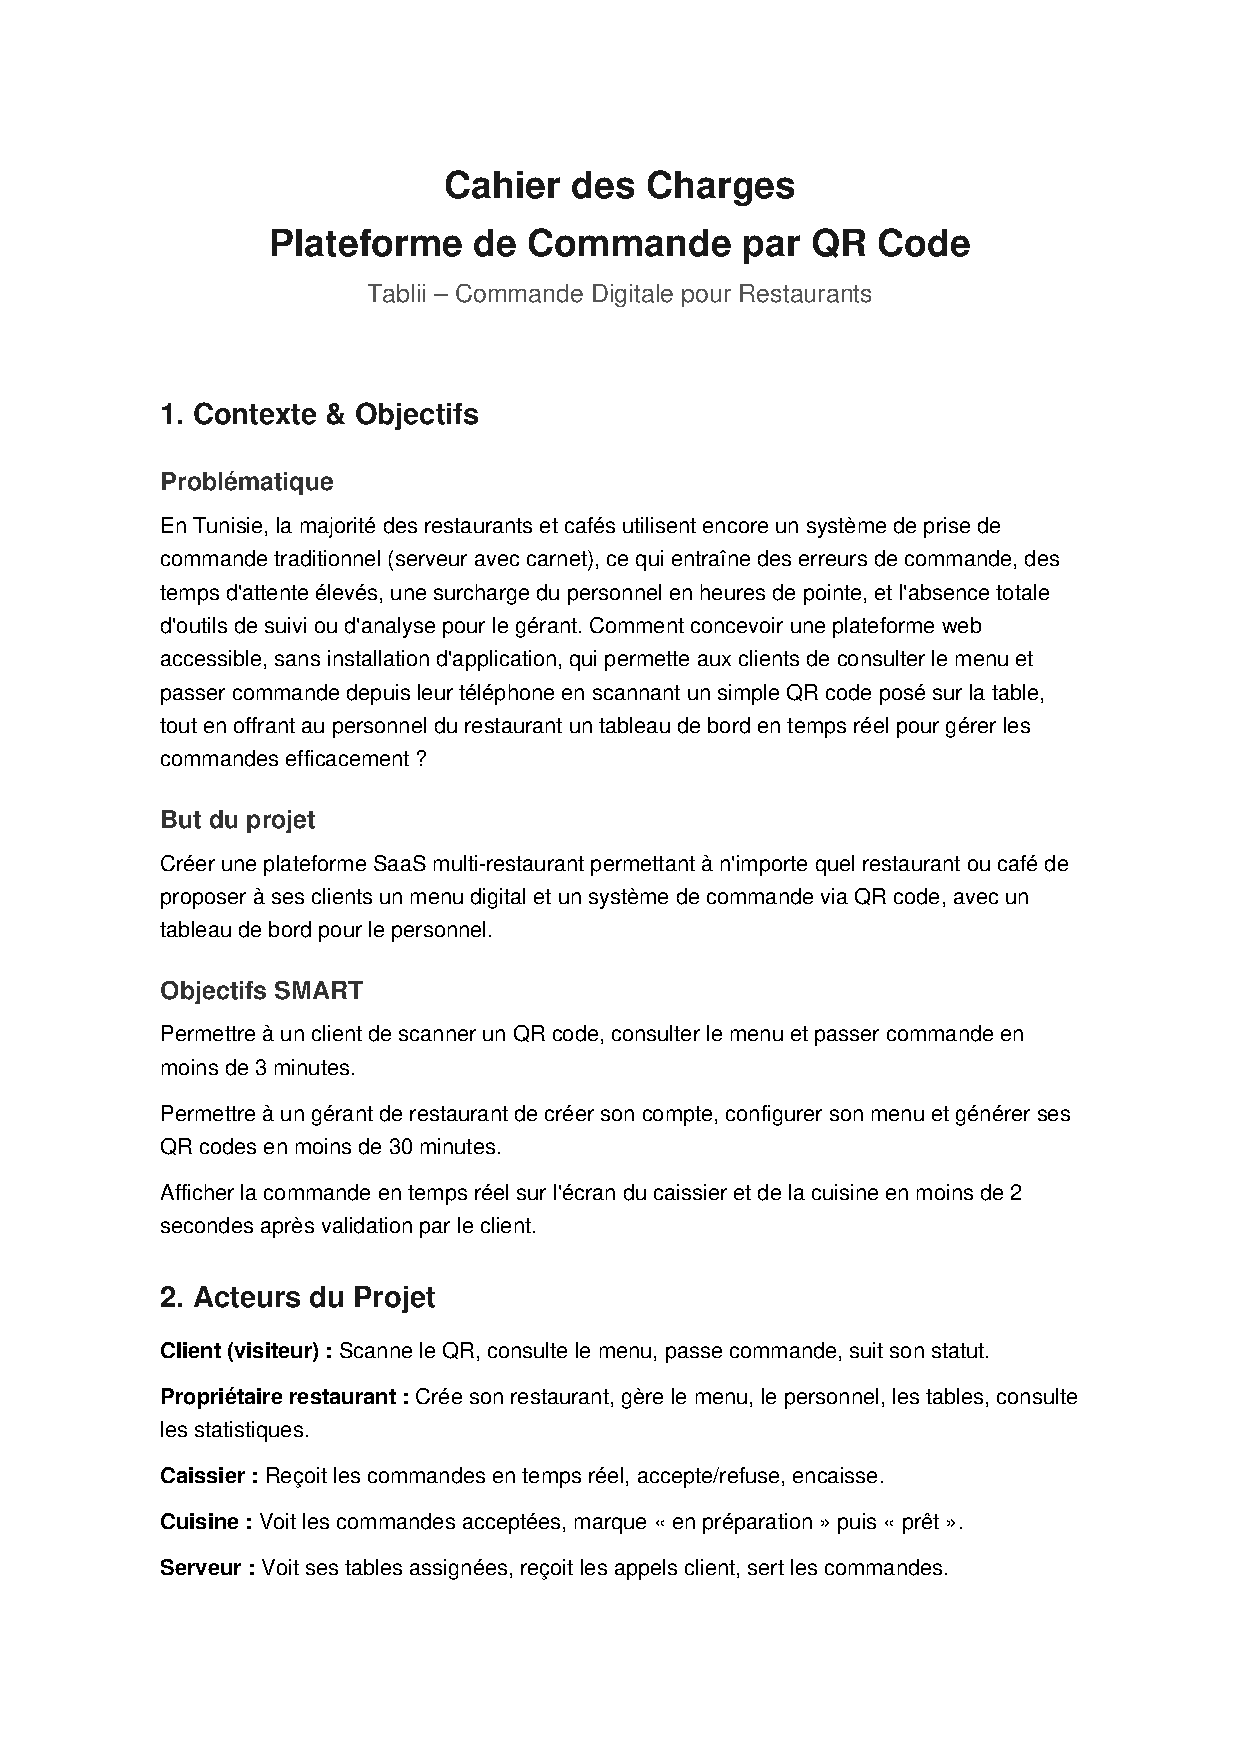
\includepdf[pages=-,scale=0.92,pagecommand={\thispagestyle{fancy}}]{resources/cahier_des_charges_tablii.pdf}
}{%
    \begin{designbox}[Cahier des charges non trouvé]
    Le fichier \resourcepath{resources/cahier\_des\_charges\_tablii.pdf} doit être présent dans le dossier \resourcepath{pfe/resources/} pour compiler cette annexe.
    \end{designbox}
}

\end{document}
